\textit{Response.} 

We begin by examining a simplified form of the given stochastic differential equation (SDE), specifically

\begin{equation}
	du^{*} = -\widehat{\gamma}\,u^{*}\,dt + \sigma_u\,dW_u,
\end{equation}

which is equivalent to the given SDE with $\omega = 0$ and $\sigma_{\gamma} = 0$ after a long time. Note that since $\omega = 0$, $u^{*}$ stays real for any real intial condition, and its real and imaginary parts behave identically for any complex initial condition. For negative $\widehat{\gamma}$, $u^{*}$ grows exponentially. Similarly, $u^{*}$ decays exponentially for positive $\widehat{\gamma}$. For $\widehat{\gamma} = 0$, the dynamics of $u^{*}$ is entirely dominated by the stochastic forcing.

Changing $\omega$ to a non-zero value, i.e., the dynamics of $u^{*}$ are given by

\begin{equation}
	du^{*} = \gpr{-\widehat{\gamma} + i\,\omega}\,u^{*}\,dt + \sigma_u\,dW_u,
\end{equation}

results in the real and imaginary parts of $u^{*}$ oscillating about each other, but does not affect the general trend of $\abs{u}$ growing or decaying exponentially. Using this information, we may speculate the behavior of $u$ in the full $\gpr{u,\ \gamma}$--system as $\gamma$ evolves.

The dynamics equation for $\gamma$ is that of a real-value Ornstein--Uhlenbeck process with equilibrium mean $\widehat{\gamma}$ and equilibrium variance $\frac{\sigma_{\gamma}^2}{2\,d_{\gamma}}$. Hence, after a long period of time, a given trajectory of $\gamma$ evolves as follows:

\begin{quote}
	When $\gamma$ is near $\widehat{\gamma}$, the stochastic forcing term dominates and pushes $\gamma$ `away' from $\widehat{\gamma}$. As $\gamma$ drifts away from $\widehat{\gamma}$, the decay term begins to dominate, and `drags' $\gamma$ back toward $\widehat{\gamma}$. This results in $\gamma$ `oscillating' irregularly about $\widehat{\gamma}$.
\end{quote}

In general, therefore, we may focus on the equilbrium distribution of $\gamma$, which is normal with mean $\widehat{\gamma}$ and variance $\frac{\sigma_{\gamma}^2}{2\,d_{\gamma}}$. We formulate the following strategy for selecting parameters to obtain the desired dynamical regimes:

\begin{enumerate}[(i)]
	\item To obtain short-lasting transient instabilities of $\func{u}{t}$, we may have $\gamma$ oscillate rapidly about zero. For this, we may select a large decay parameter $d_{\gamma}$, small stochastic forcing strength $\sigma_{\gamma}$, and small equilibrium mean $\widehat{\gamma}$ for $\gamma$. The value for $\omega$ and $\sigma_u$ are not as important. In the figures below, we use the following parameters
	
	\begin{equation}
		\omega = 1,\qquad \sigma_u = 0.5,\qquad d_{\gamma} = 4.8,\qquad \widehat{\gamma} = 0.1,\qquad \sigma_{\gamma} = 1.2,
	\end{equation}
	
	which results in $\gamma_{eq} \sim \func{\mathcal{N}}{0.1,\ 0.387}$, i.e., $\gamma$ is negative with probability 0.398 and positive with probability 0.602.
	
	\begin{figure}[H]
		\centering
		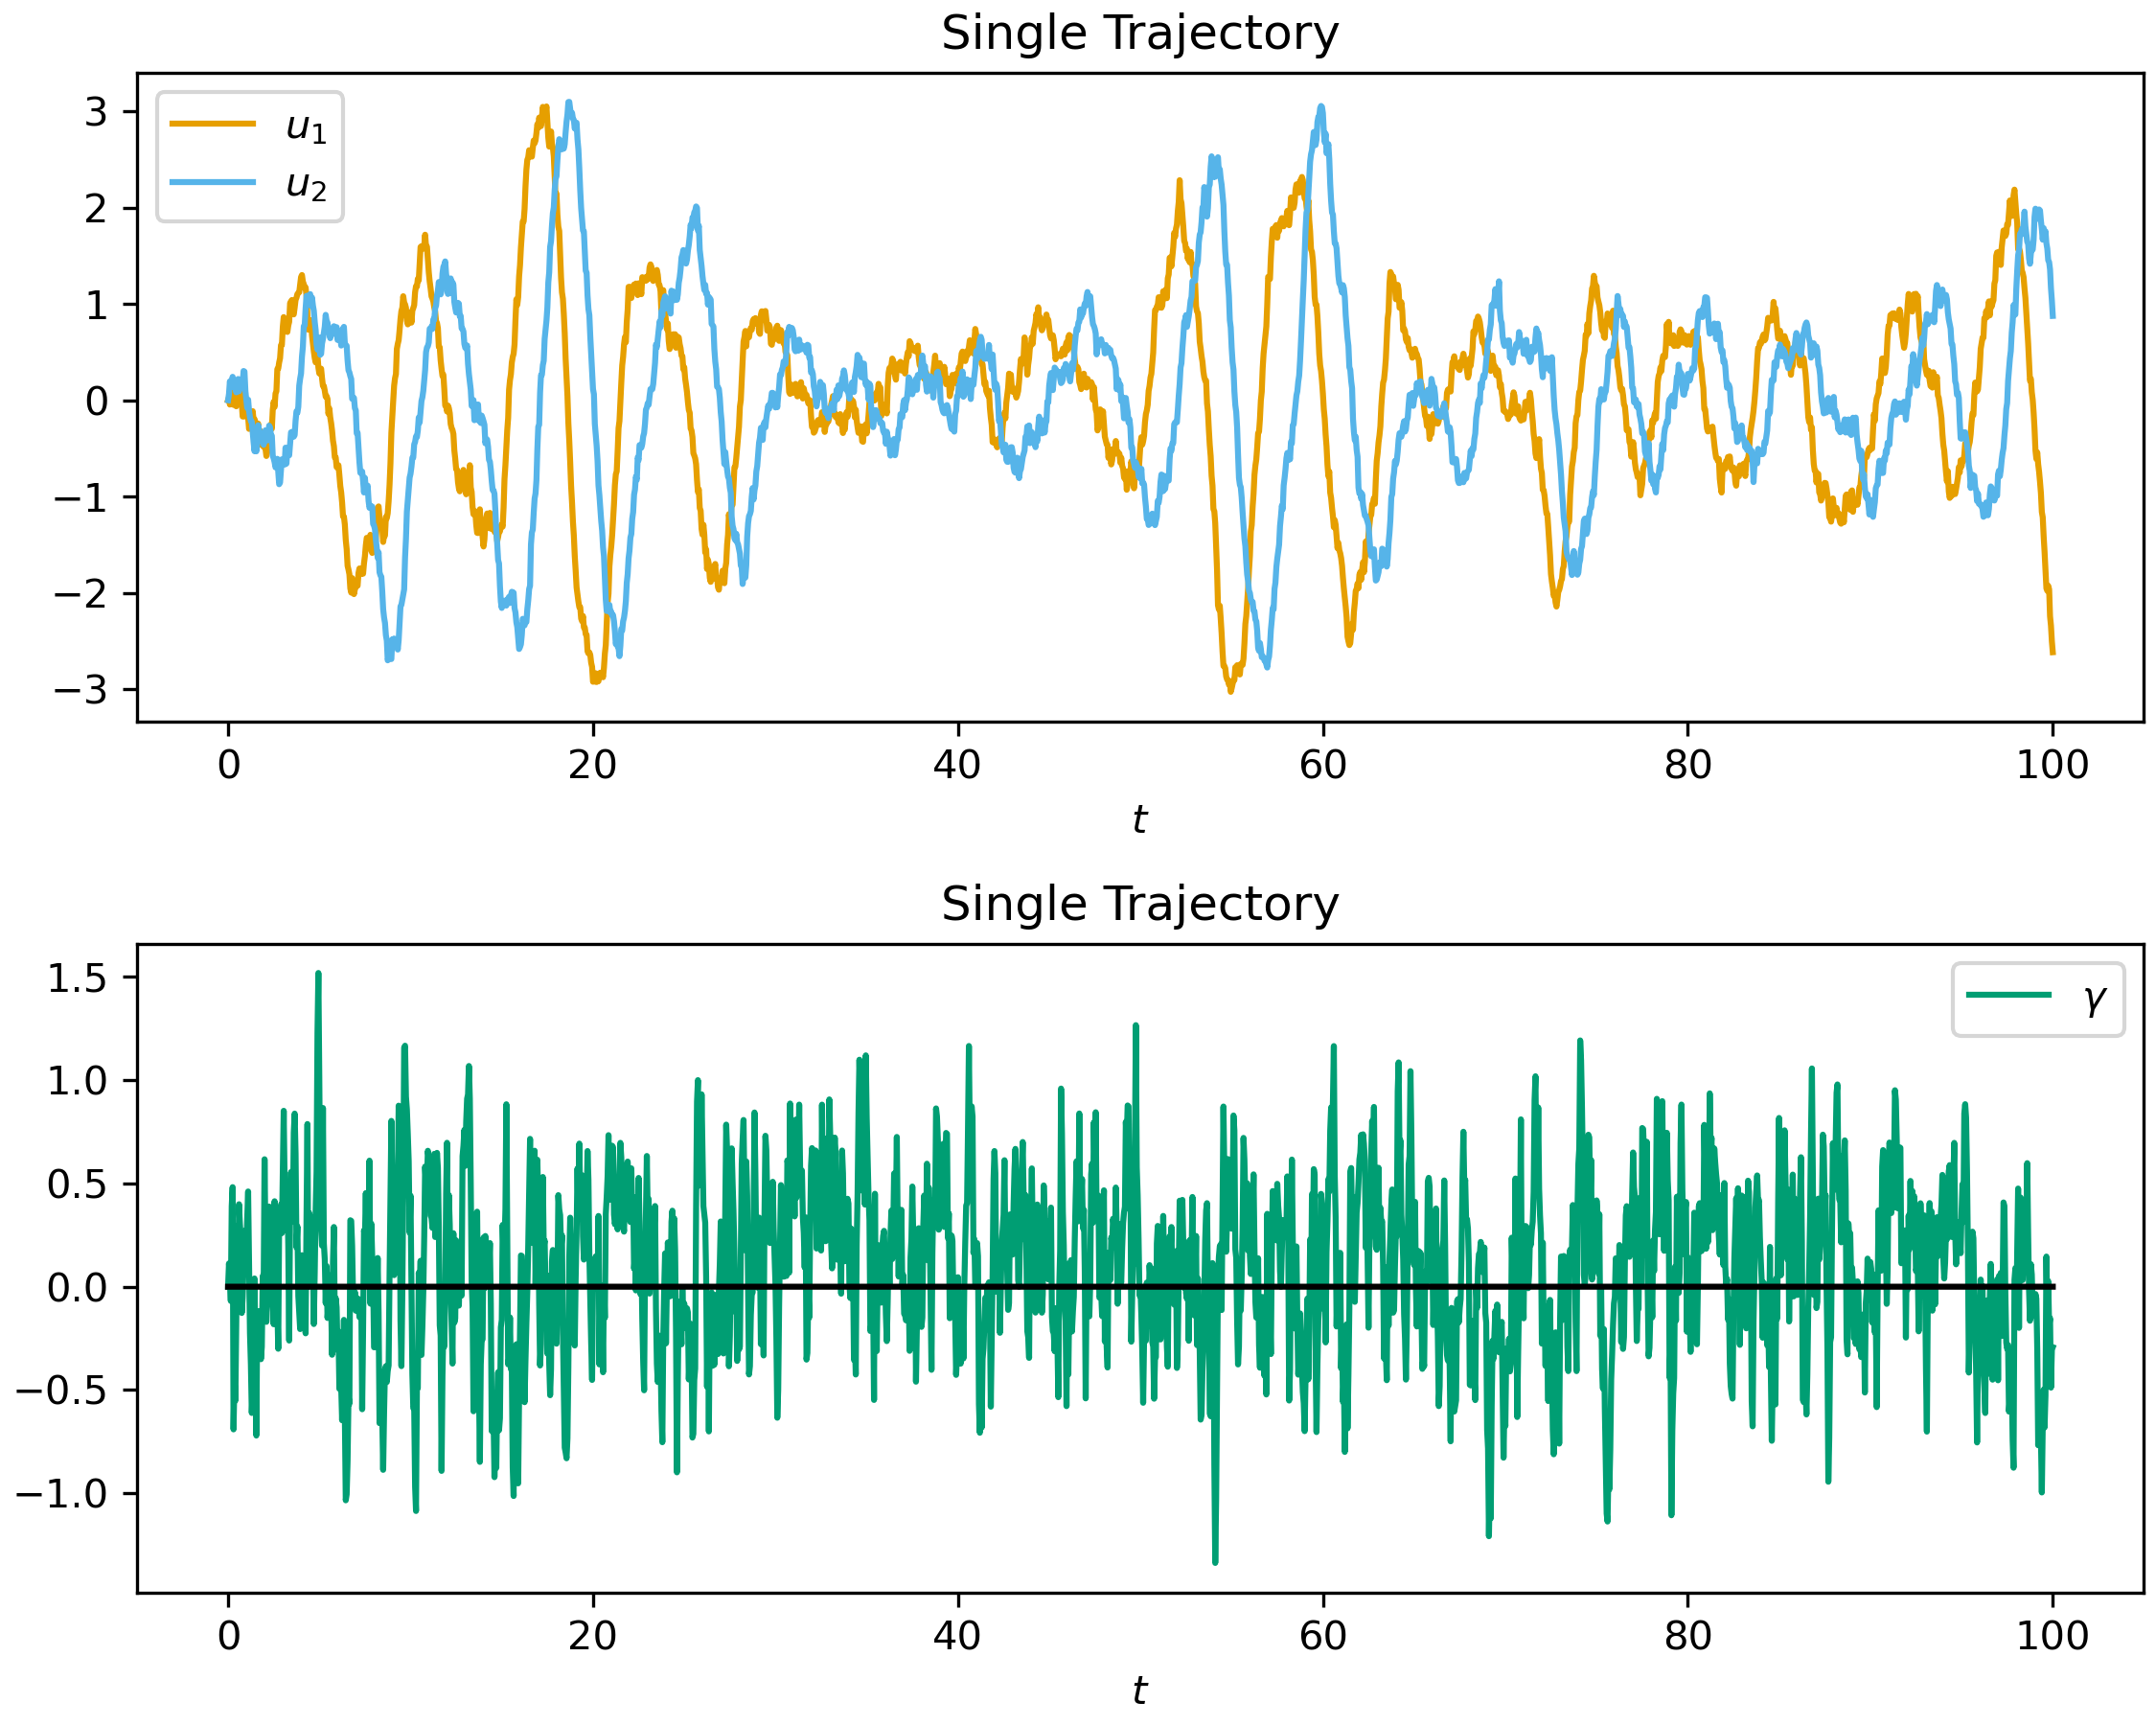
\includegraphics[width=0.75\textwidth]{../../src/2_traj_i.png}
		\caption{A single realization of the linear SDE with multiplicative noise with the parameters $\omega = 1$, $\sigma_u = 0.5$, $d_{\gamma} = 4.8$, $\widehat{\gamma} = 0.1$, and $\sigma_{\gamma} = 1.2$ with initial condition $u = u_1 + i\,u_2 = v = 0$. For clarity of deciphering when $u_1$, $u_2$ are in a stable or unstable regime, we include a solid black line at $\gamma = 0$.}
		\label{fig:2_traj_i}
	\end{figure}
	
	\begin{figure}[H]
		\centering
		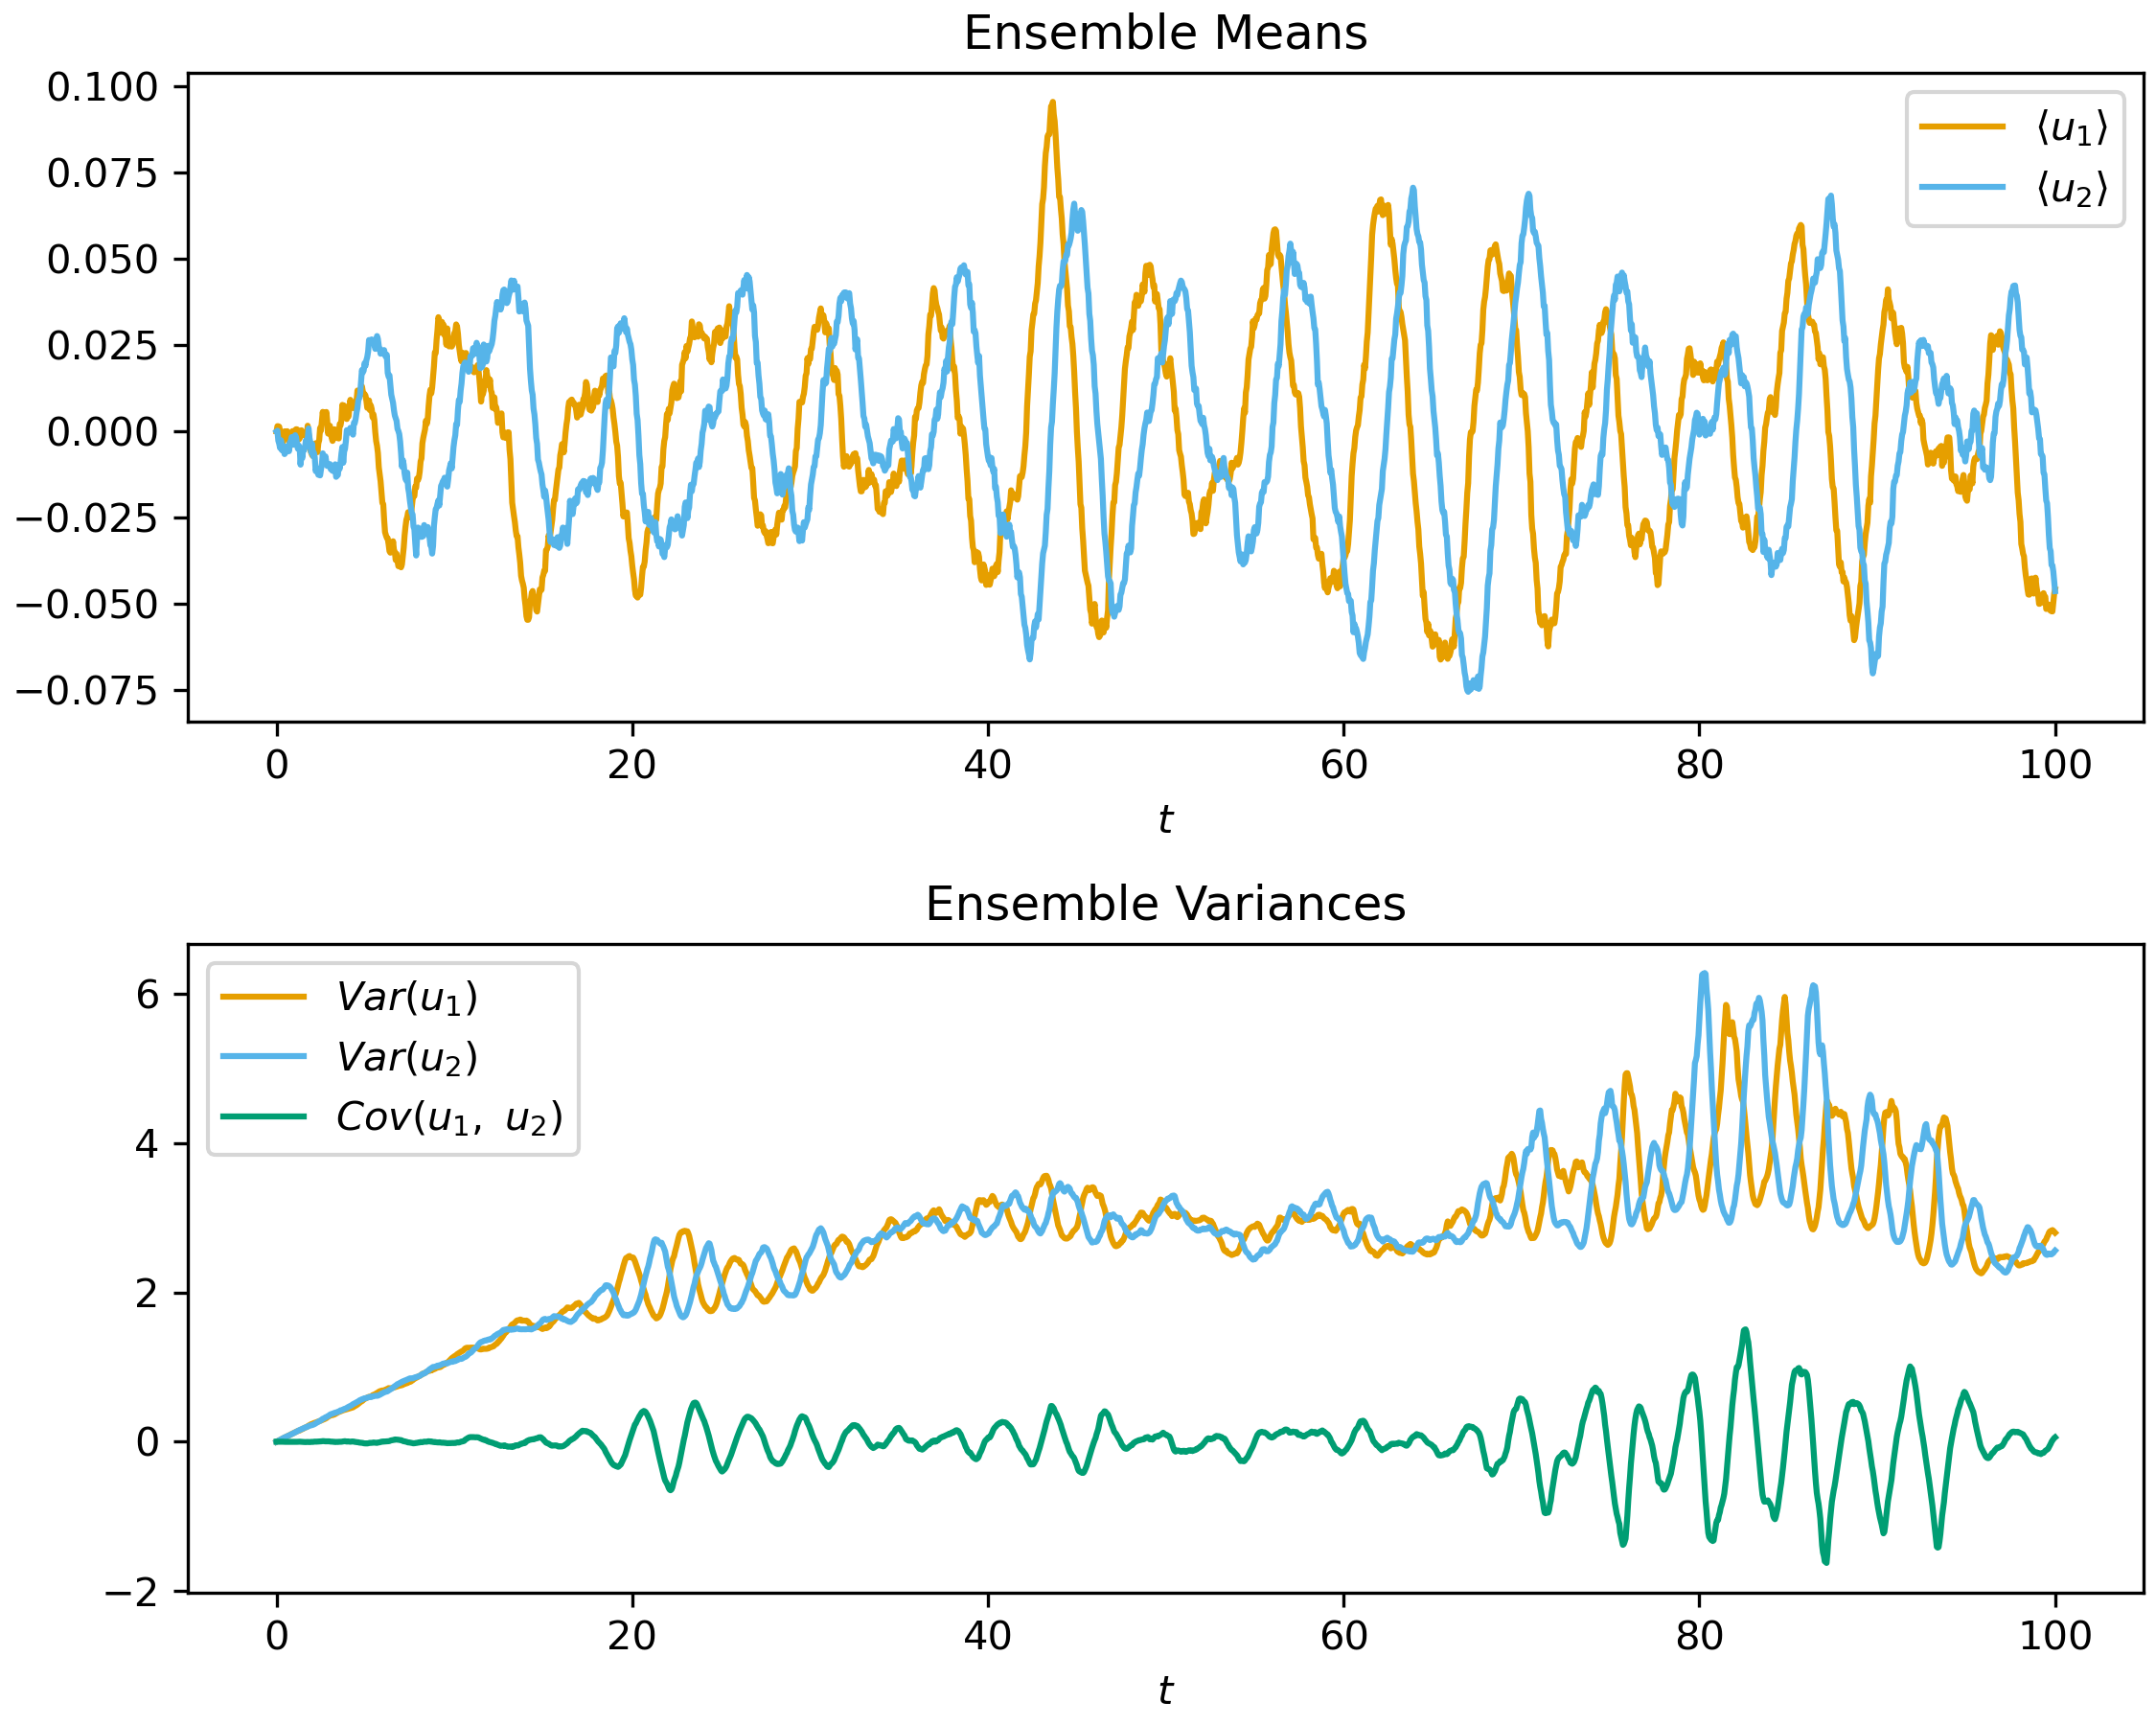
\includegraphics[width=0.75\textwidth]{../../src/2_ens_stats_i.png}
		\caption{The ensemble statistics for 1000 realizations of the linear SDE with multiplicative noise with the parameters $\omega = 1$, $\sigma_u = 0.5$, $d_{\gamma} = 4.8$, $\widehat{\gamma} = 0.1$, and $\sigma_{\gamma} = 1.2$ with initial condition $u = u_1 + i\,u_2 = v = 0$ for each realization.}
		\label{fig:2_ens_stats_i}
	\end{figure}
	
	\begin{figure}[H]
		\centering
		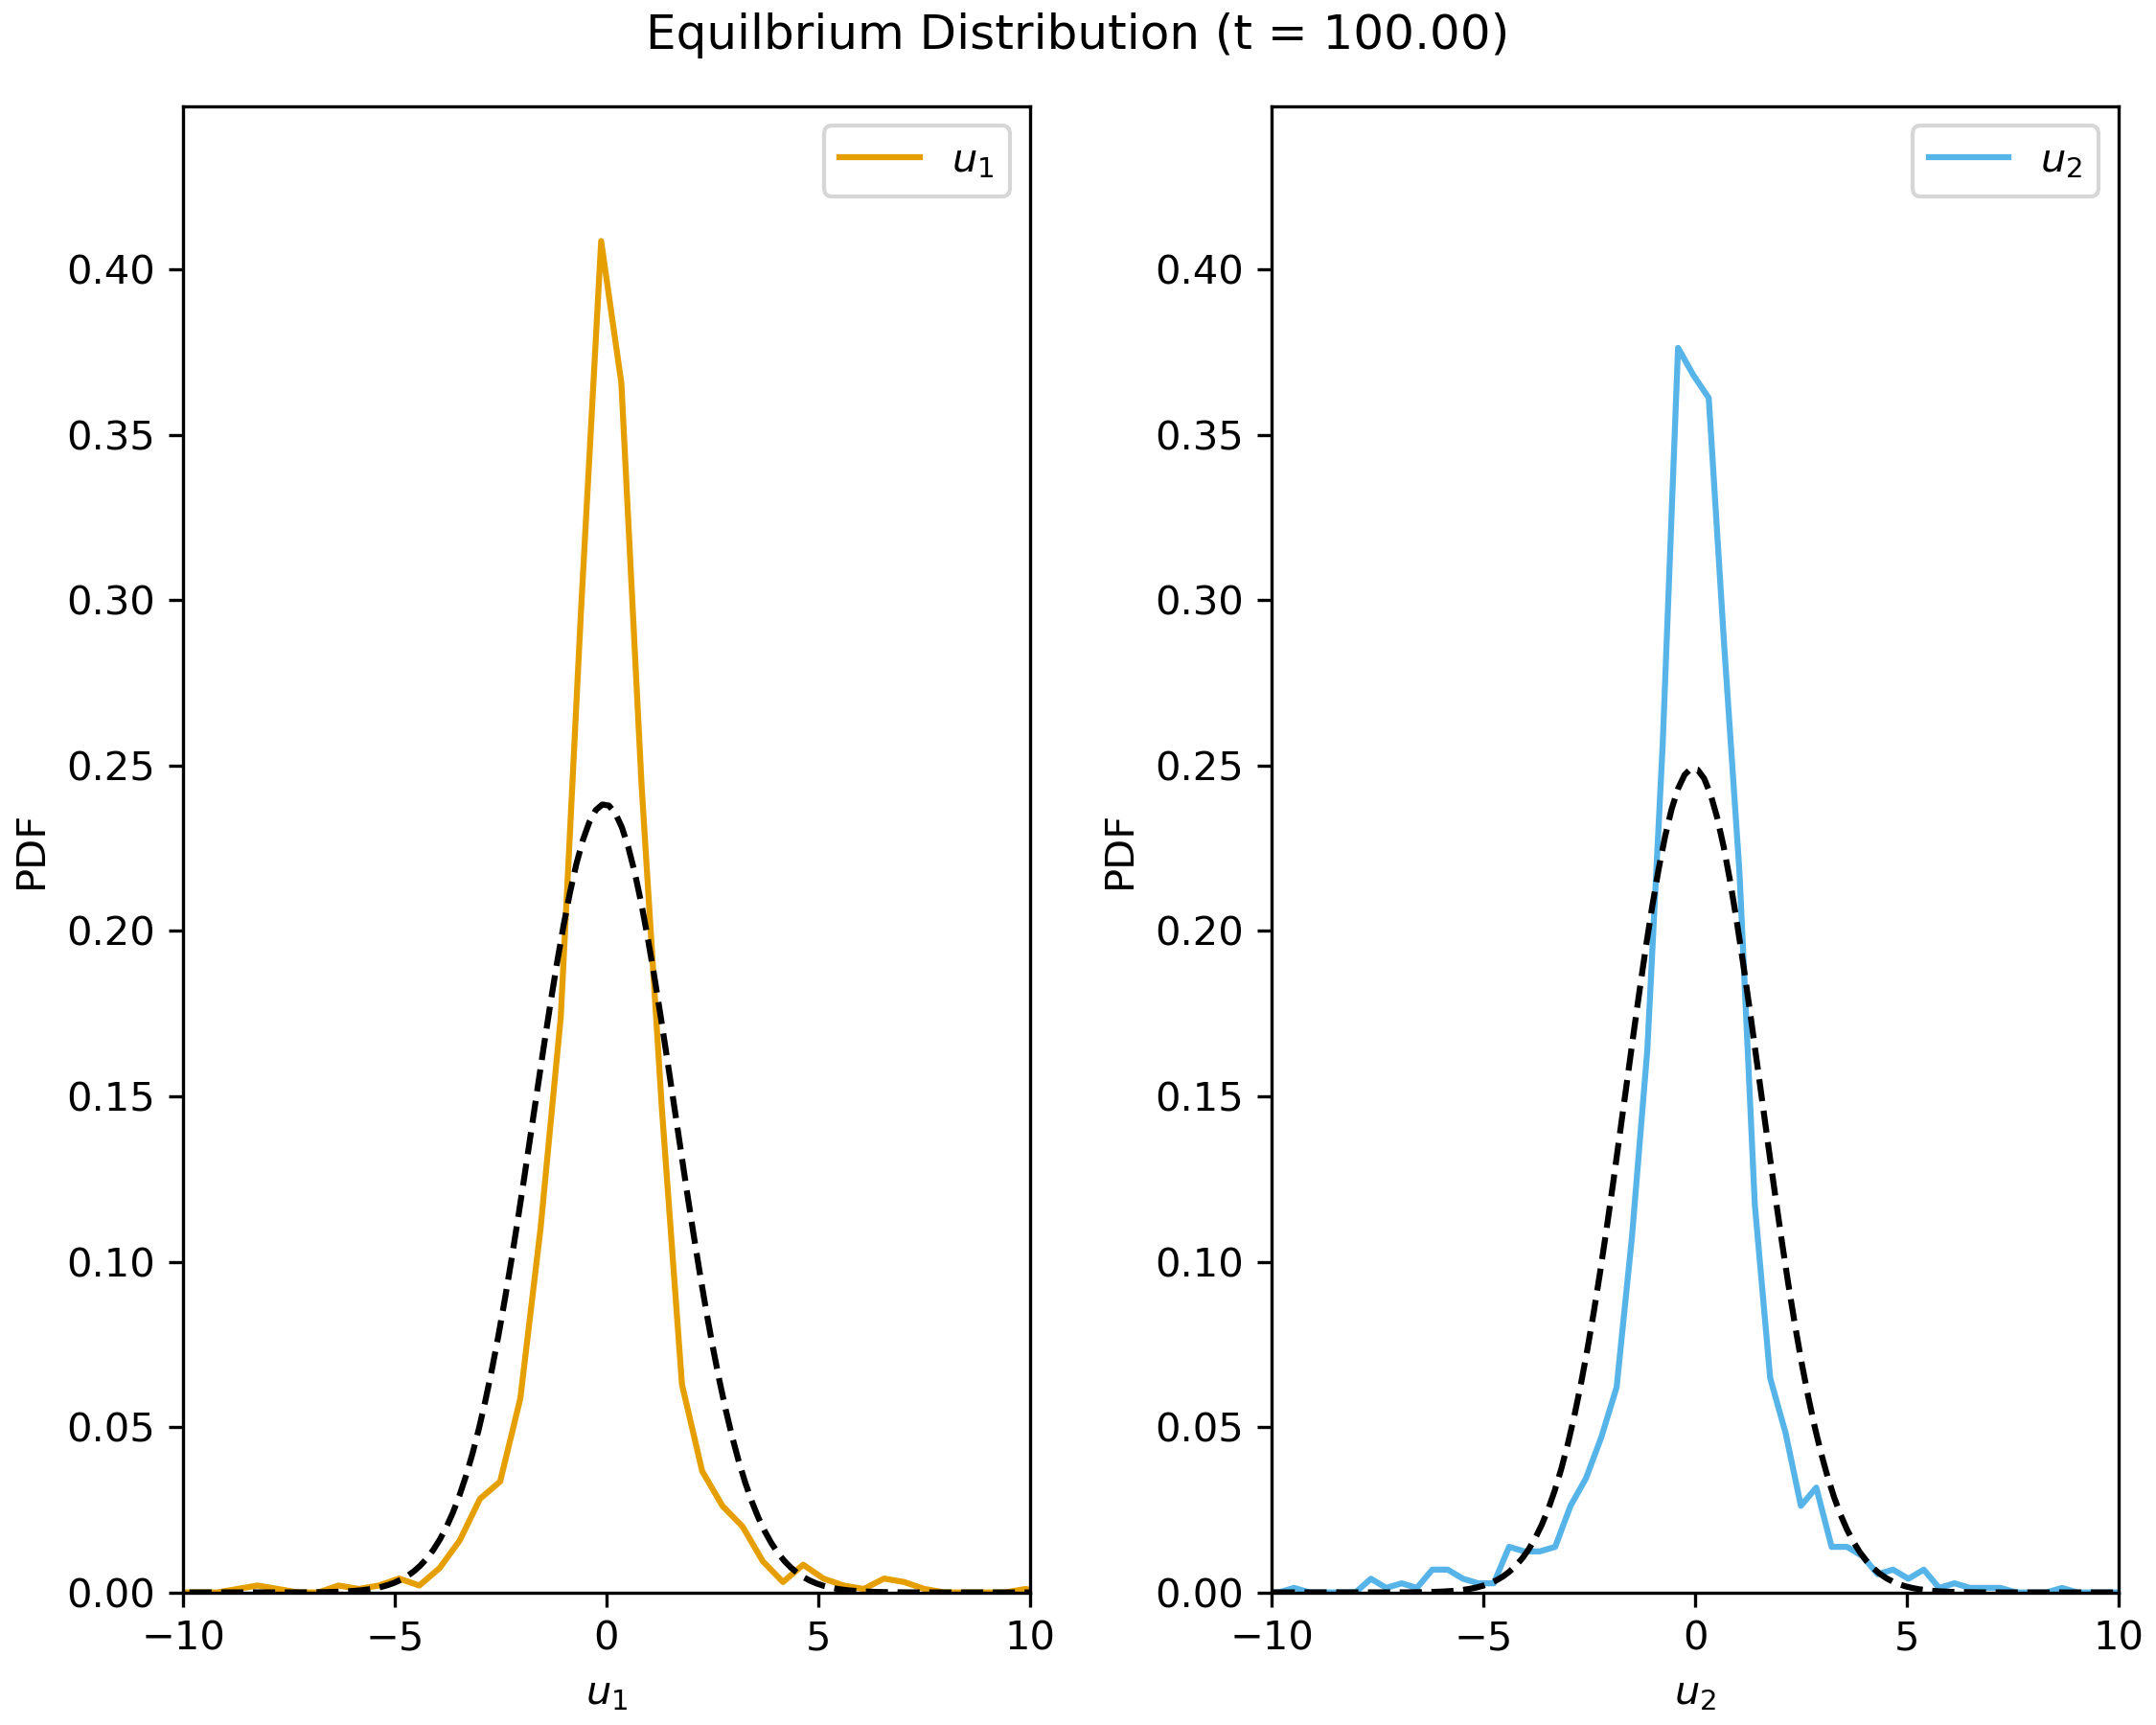
\includegraphics[width=0.75\textwidth]{../../src/2_equ_pdf_i.png}
		\caption{The equilibrium distribution for 1000 realizations of the linear SDE with multiplicative noise with the parameters $\omega = 1$, $\sigma_u = 0.5$, $d_{\gamma} = 4.8$, $\widehat{\gamma} = 0.1$, and $\sigma_{\gamma} = 1.2$ with initial condition $u = u_1 + i\,u_2 = v = 0$ for each realization. The dashed black line corresponds to a Gaussian fit for the data.}
		\label{fig:2_equ_pdf_i}
	\end{figure}
	
	\begin{figure}[H]
		\centering
		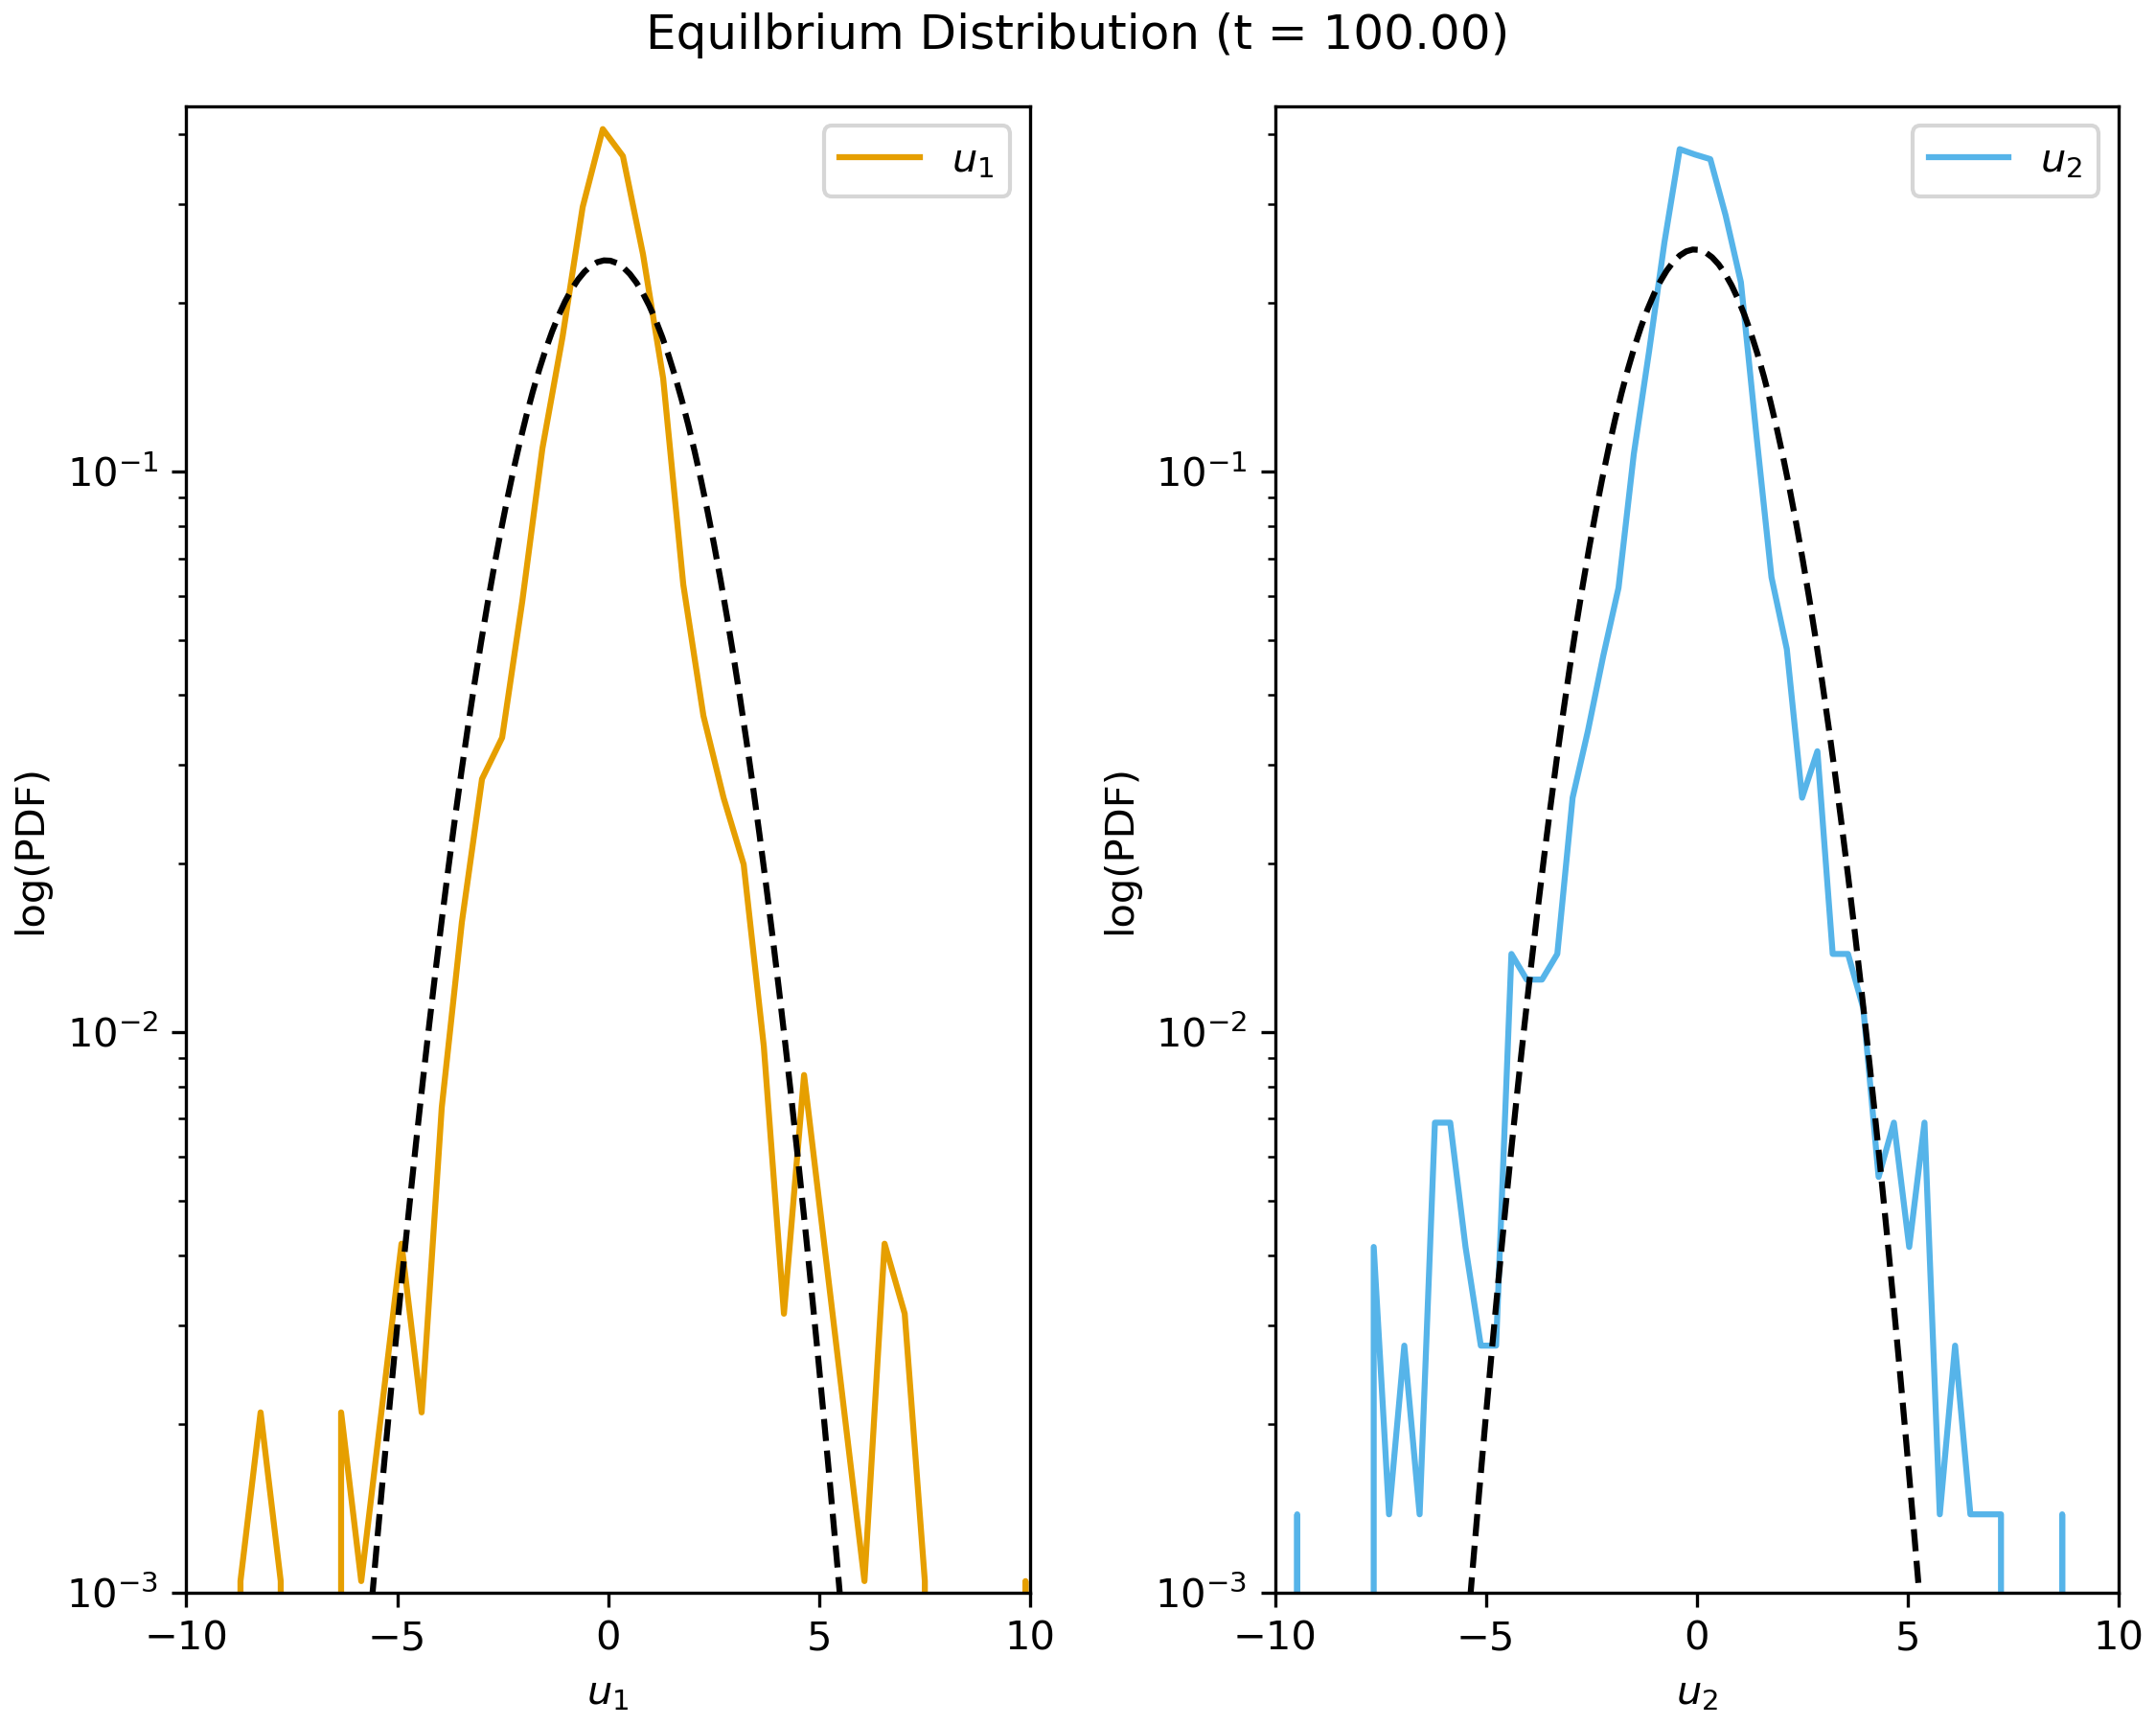
\includegraphics[width=0.75\textwidth]{../../src/2_log_equ_pdf_i.png}
		\caption{The log of the equilibrium distribution for 1000 realizations of the linear SDE with multiplicative noise with the parameters $\omega = 1$, $\sigma_u = 0.5$, $d_{\gamma} = 4.8$, $\widehat{\gamma} = 0.1$, and $\sigma_{\gamma} = 1.2$ with initial condition $u = u_1 + i\,u_2 = v = 0$ for each realization. The dashed black line corresponds to a Gaussian fit for the data.}
		\label{fig:2_log_equ_pdf_i}
	\end{figure}
	
	\item To obtain intermittent large-amplitude instabilities of $\func{u}{t}$, we may have $\gamma$ oscillate more slowly around zero. In particular, we wish for $\gamma$ to generally be positive with small deviations below zero. For this, we may select a small decay parameter $d_{\gamma}$, large stochastic forcing strength $\sigma_{\gamma}$, and large equilibrium mean $\widehat{\gamma}$ for $\gamma$. The value for $\omega$ and $\sigma_u$ are not as important. In the figure below, we use the following parameters
	
	\begin{equation}
		\omega = 1,\qquad \sigma_u = 0.5,\qquad d_{\gamma} = 0.625,\qquad \widehat{\gamma} = 3,\qquad \sigma_{\gamma} = 2,
	\end{equation}
	
	which results in $\gamma_{eq} \sim \func{\mathcal{N}}{3,\ 1.789}$, i.e., $\gamma$ is negative with probability 0.0468 and positive with probability 0.9532.
	

	\begin{figure}[H]
		\centering
		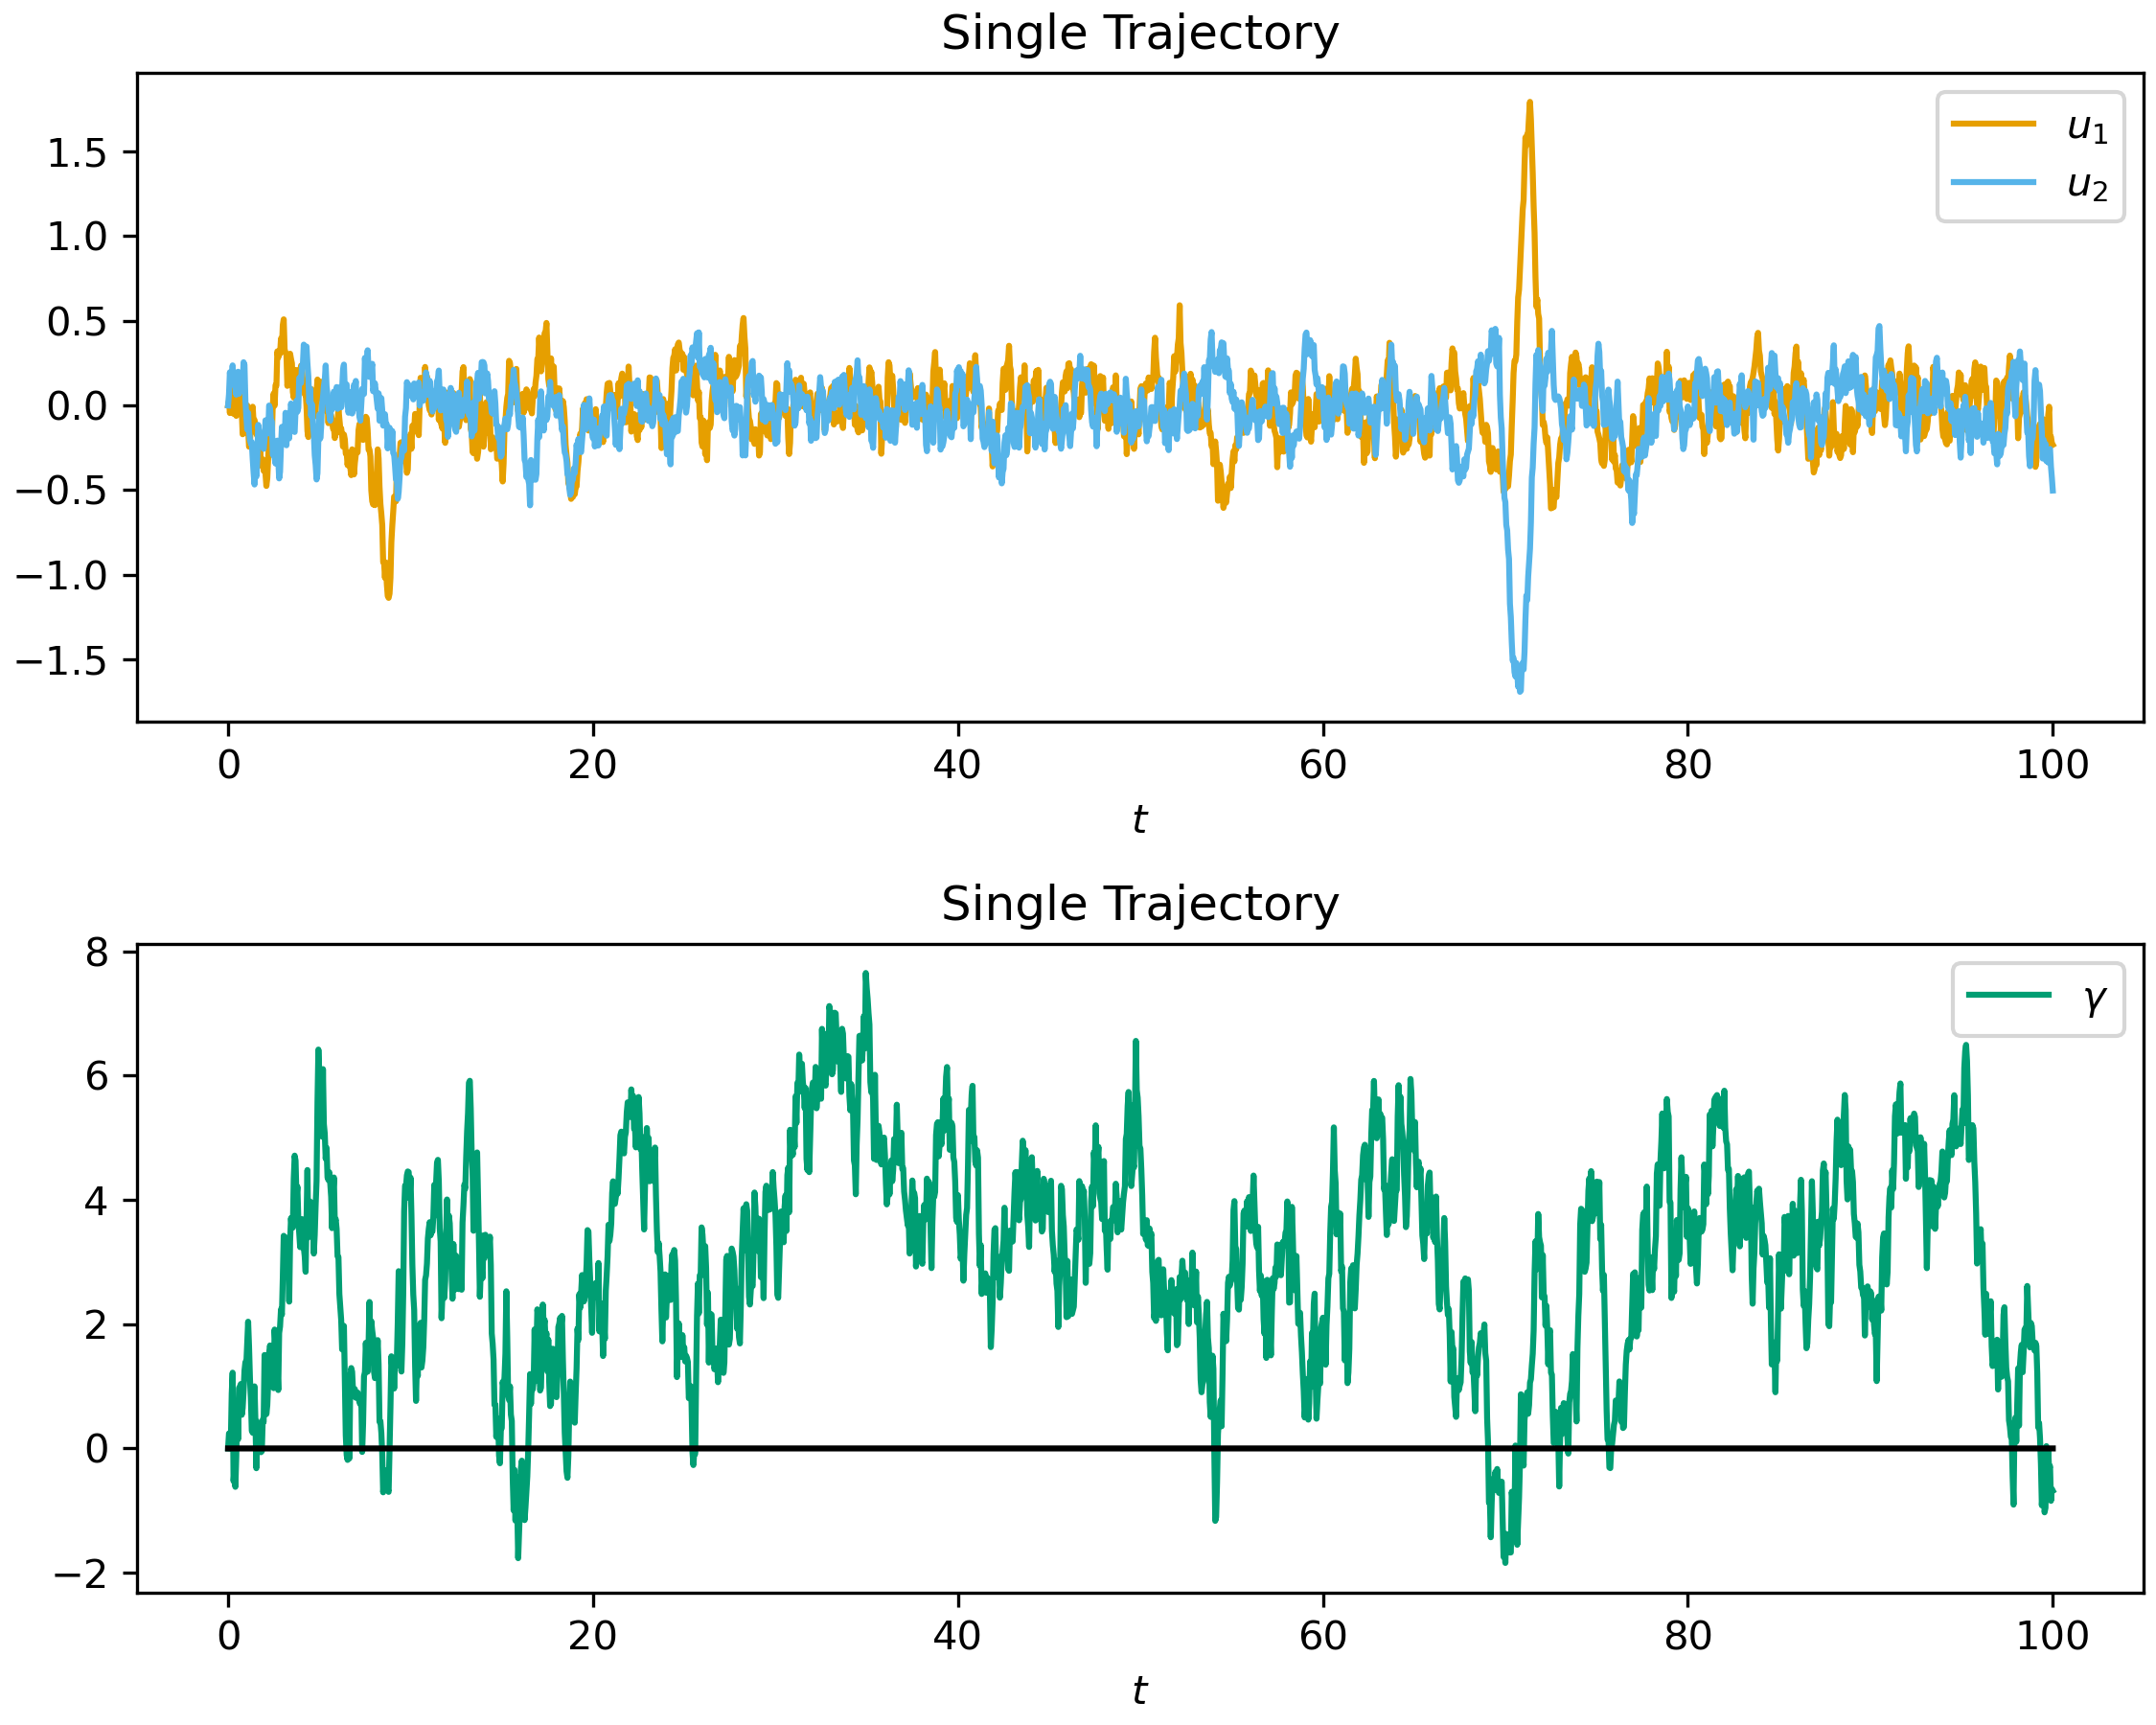
\includegraphics[width=0.75\textwidth]{../../src/2_traj_ii.png}
		\caption{A single realization of the linear SDE with multiplicative noise with the parameters $\omega = 1$, $\sigma_u = 0.5$, $d_{\gamma} = 0.625$, $\widehat{\gamma} = 3$, and $\sigma_{\gamma} = 2$ with initial condition $u = u_1 + i\,u_2 = v = 0$. For clarity of deciphering when $u_1$, $u_2$ are in a stable or unstable regime, we include a solid black line at $\gamma = 0$.}
		\label{fig:2_traj_ii}
	\end{figure}

	\begin{figure}[H]
		\centering
		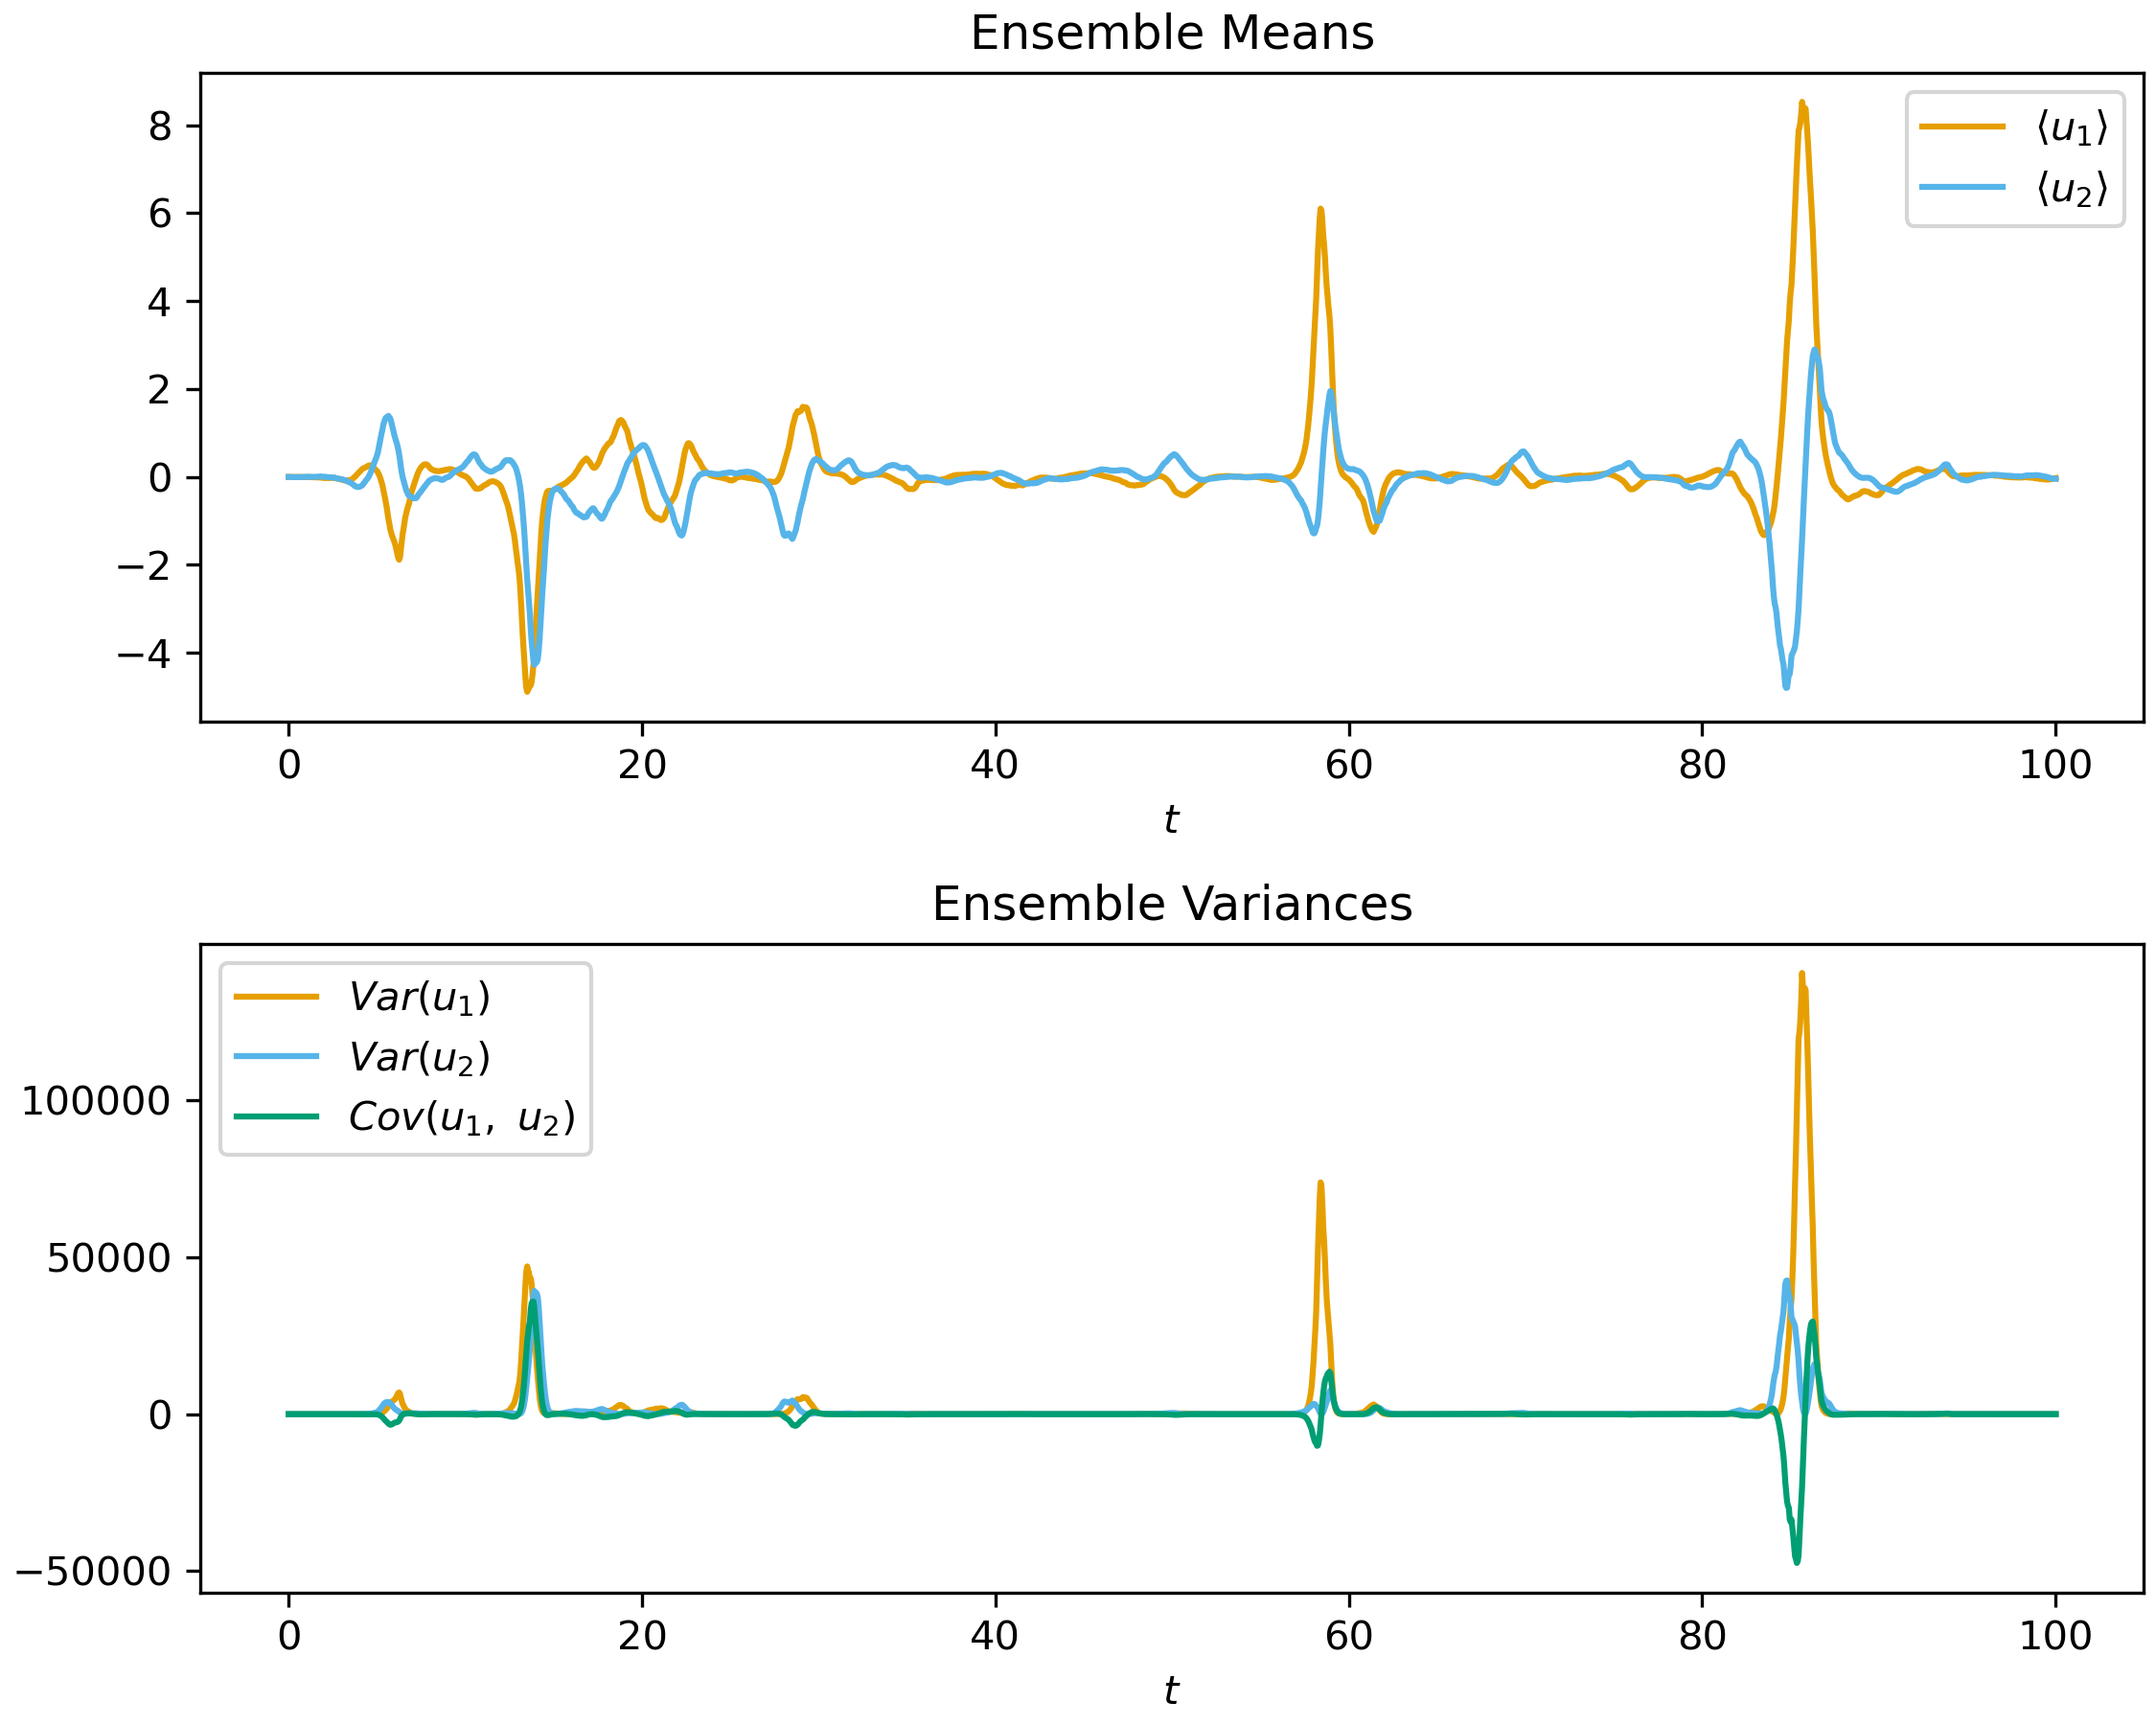
\includegraphics[width=0.75\textwidth]{../../src/2_ens_stats_ii.png}
		\caption{The ensemble statistics for 1000 realizations of the linear SDE with multiplicative noise with the parameters $\omega = 1$, $\sigma_u = 0.5$, $d_{\gamma} = 0.625$, $\widehat{\gamma} = 3$, and $\sigma_{\gamma} = 2$ with initial condition $u = u_1 + i\,u_2 = v = 0$ for each realization.}
		\label{fig:2_ens_stats_ii}
	\end{figure}
	
	\begin{figure}[H]
		\centering
		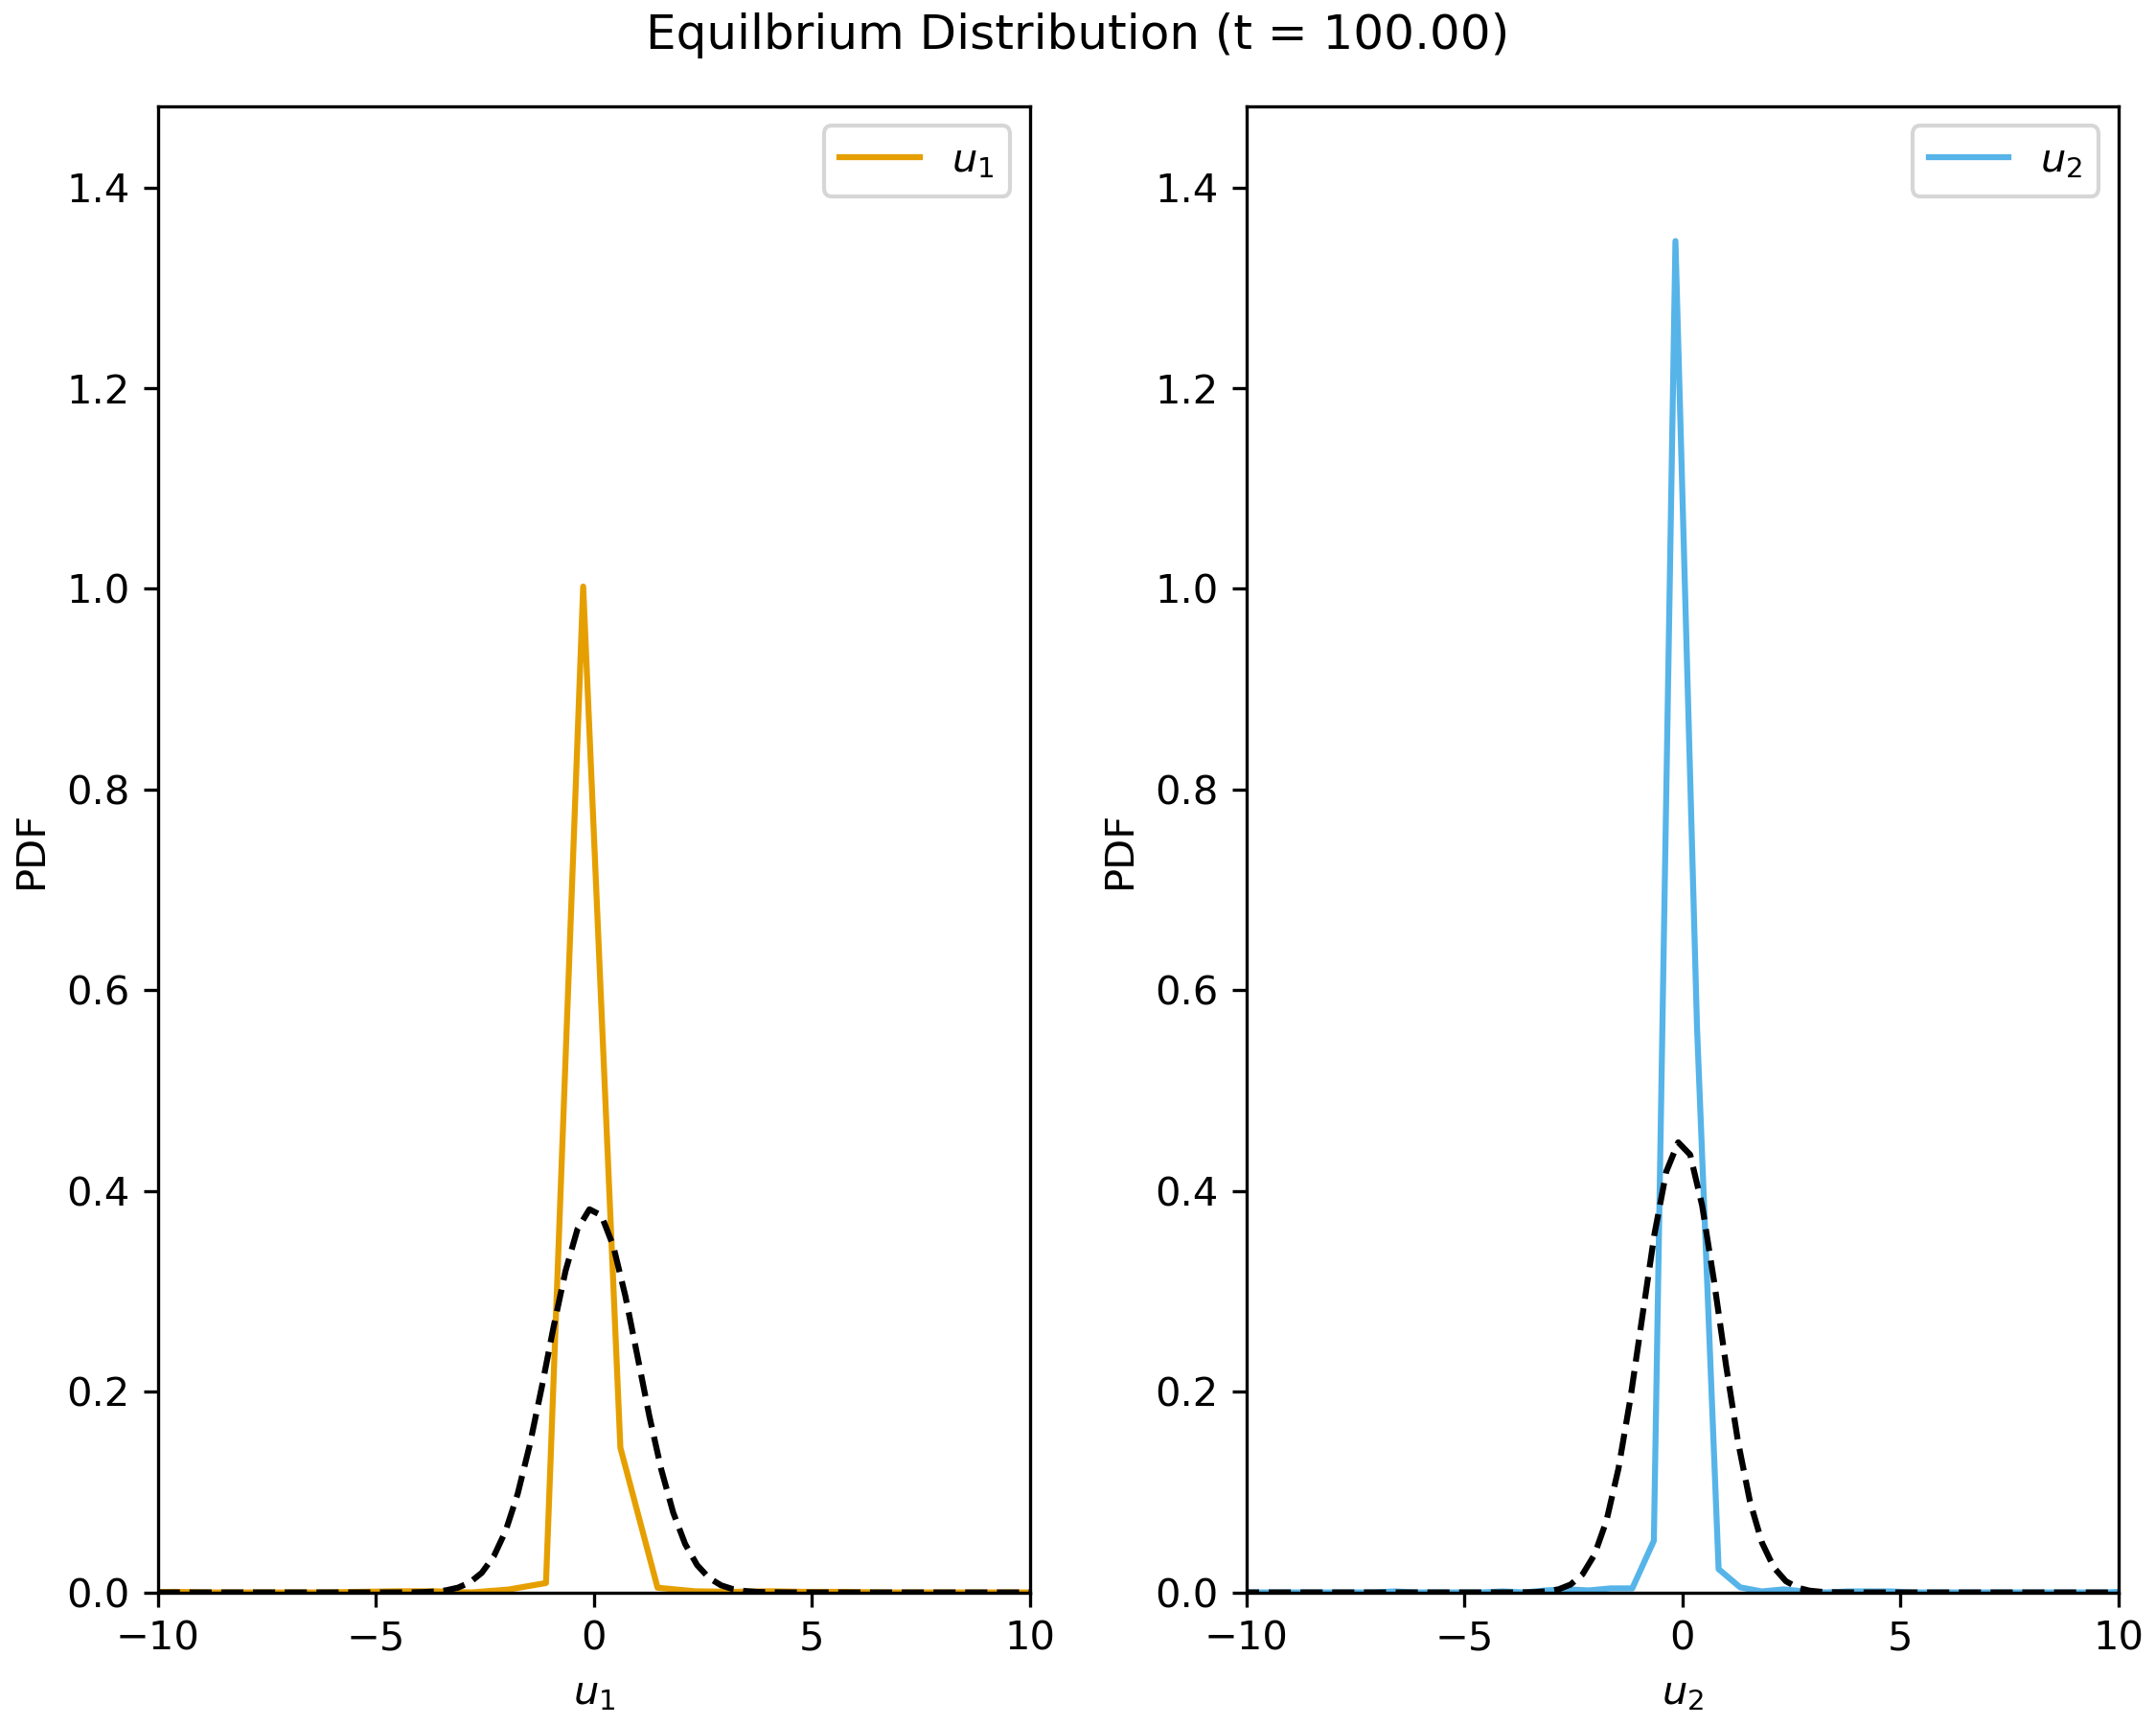
\includegraphics[width=0.75\textwidth]{../../src/2_equ_pdf_ii.png}
		\caption{The equilibrium distribution for 1000 realizations of the linear SDE with multiplicative noise with the parameters $\omega = 1$, $\sigma_u = 0.5$, $d_{\gamma} = 0.625$, $\widehat{\gamma} = 3$, and $\sigma_{\gamma} = 2$ with initial condition $u = u_1 + i\,u_2 = v = 0$ for each realization. The dashed black line corresponds to a Gaussian fit for the data.}
		\label{fig:2_equ_pdf_ii}
	\end{figure}
	
	\begin{figure}[H]
		\centering
		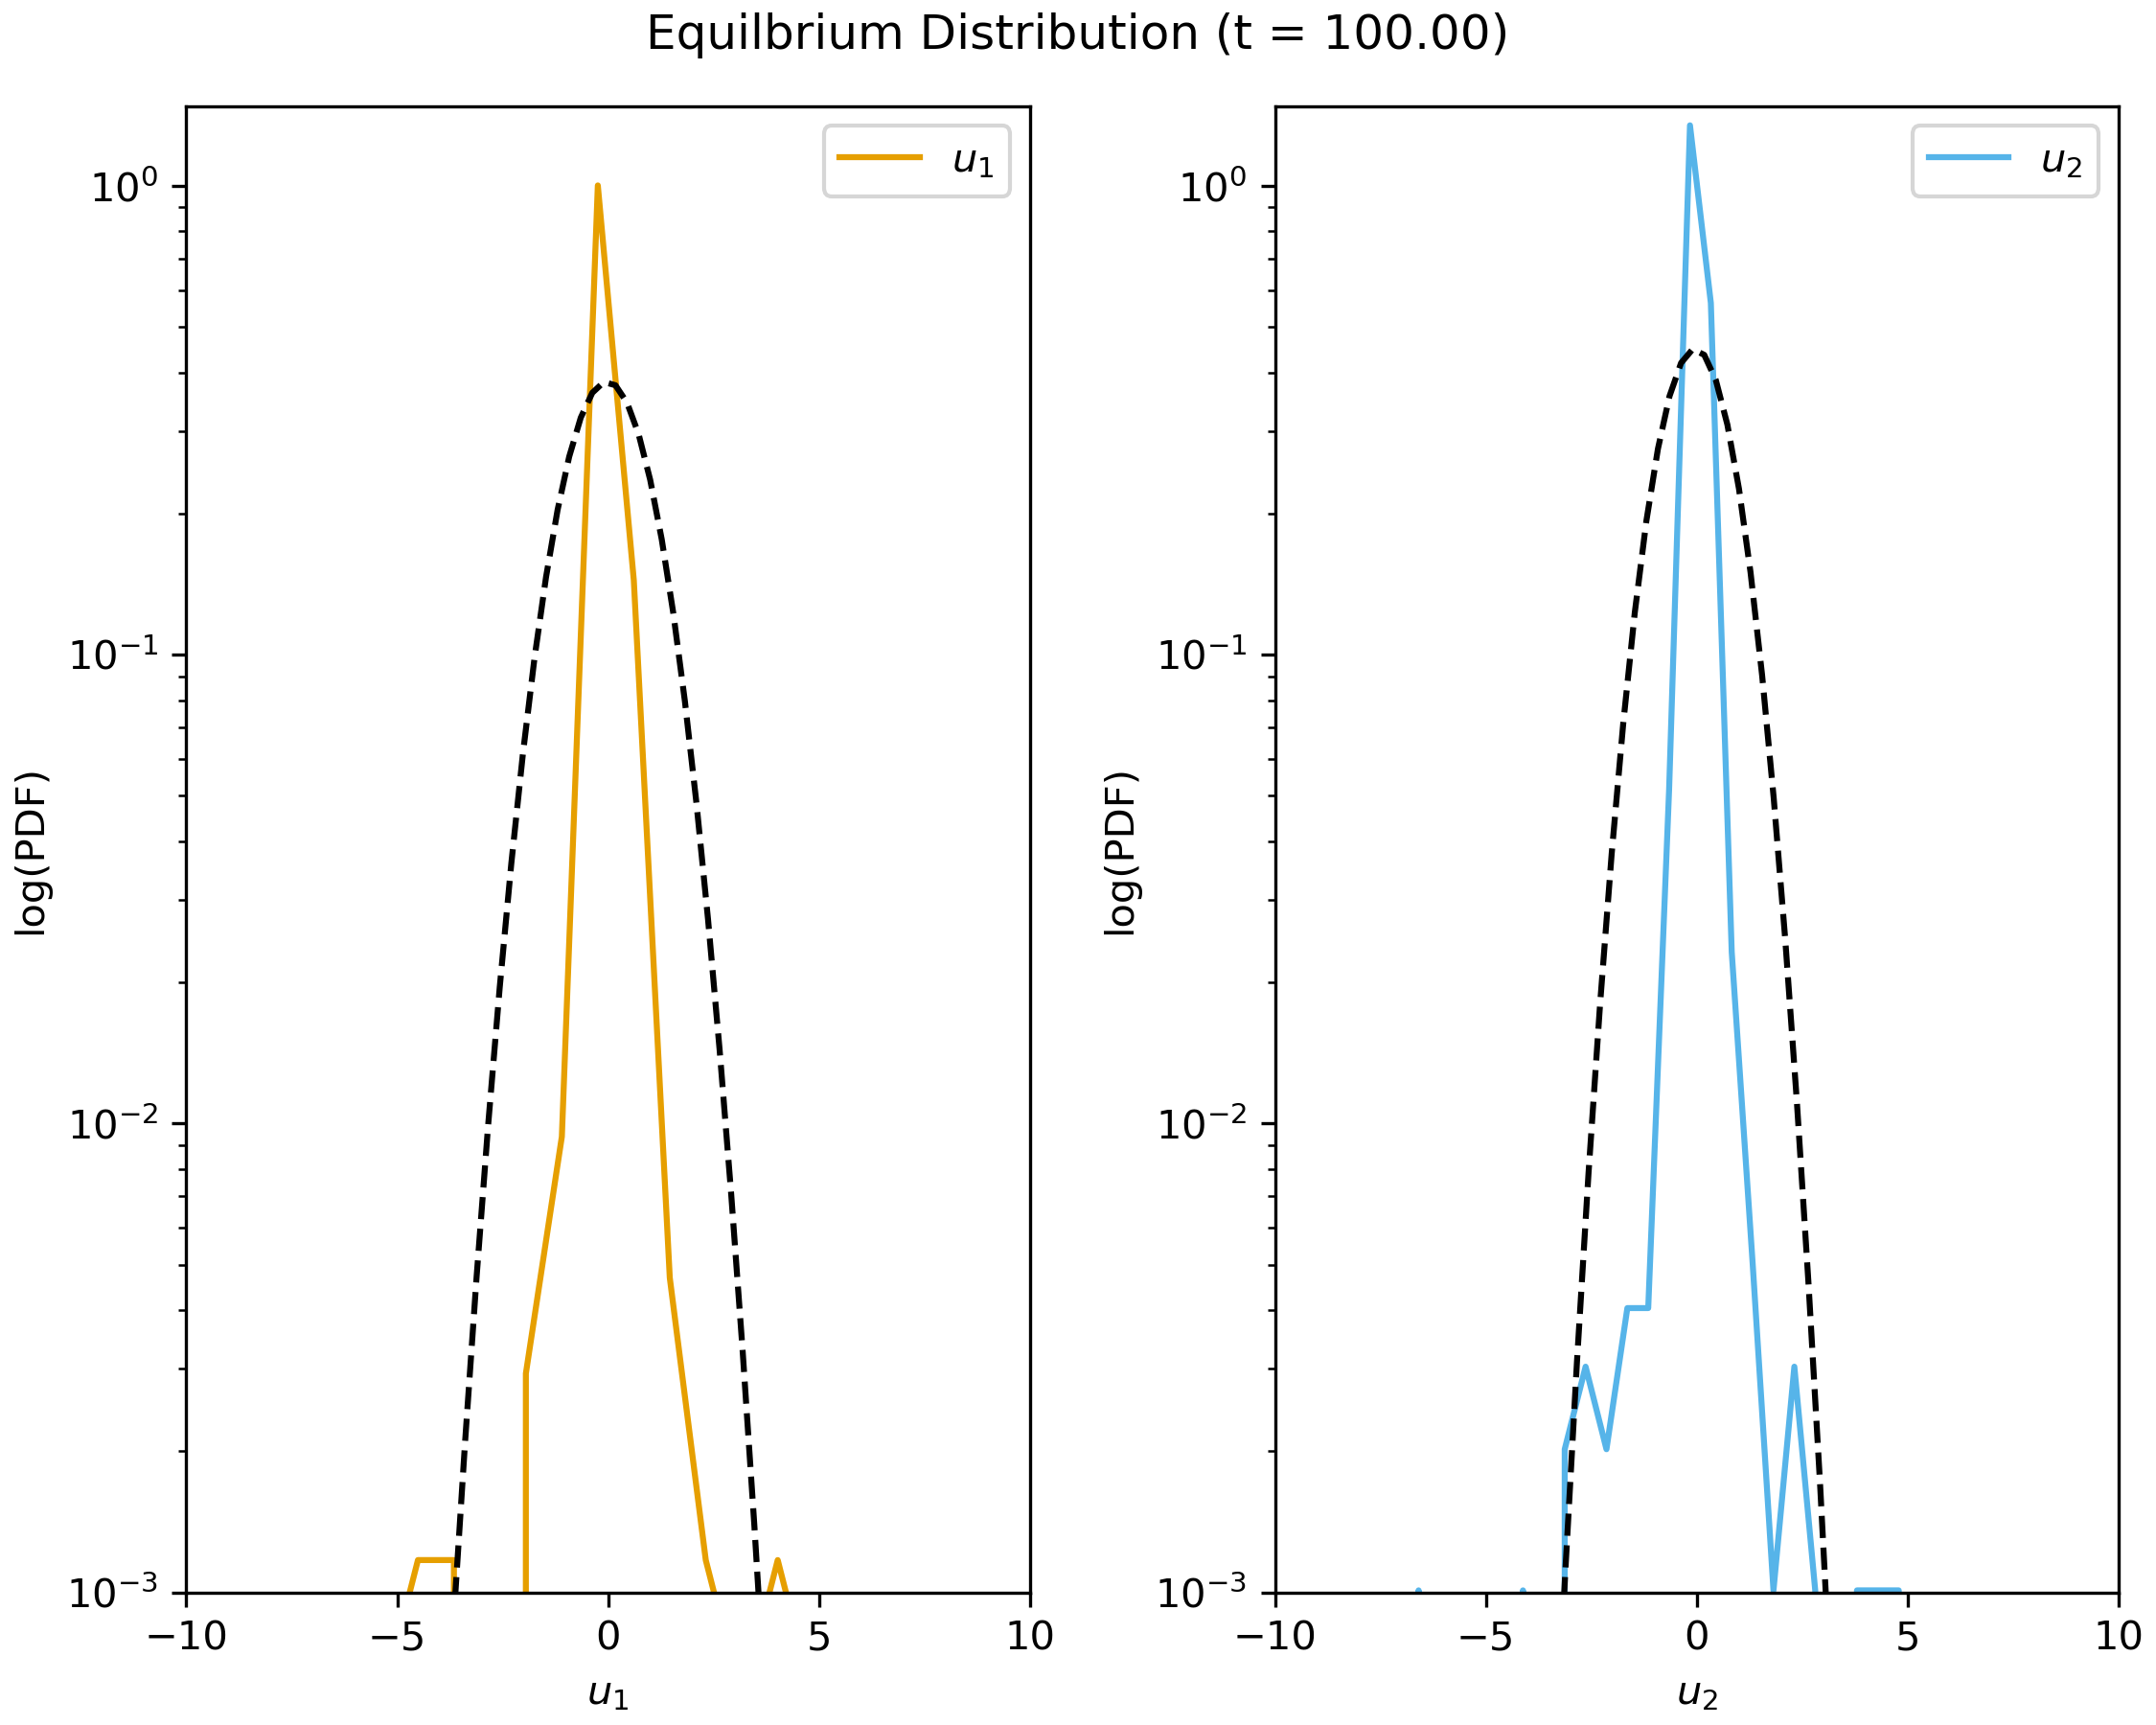
\includegraphics[width=0.75\textwidth]{../../src/2_log_equ_pdf_ii.png}
		\caption{The log of the equilibrium distribution for 1000 realizations of the linear SDE with multiplicative noise with the parameters $\omega = 1$, $\sigma_u = 0.5$, $d_{\gamma} = 0.625$, $\widehat{\gamma} = 3$, and $\sigma_{\gamma} = 2$ with initial condition $u = u_1 + i\,u_2 = v = 0$ for each realization. The dashed black line corresponds to a Gaussian fit for the data.}
		\label{fig:2_log_equ_pdf_ii}
	\end{figure}
	
	\item To obtain a stable regime of $\func{u}{t}$, we may have $\gamma$ be always positive. For this, we may select a large decay parameter $d_{\gamma}$, small stochastic forcing strength $\sigma_{\gamma}$, and large positive equilibrium mean $\widehat{\gamma}$ for $\gamma$. The value for $\omega$ and $\sigma_u$ are not as important. In the figure below, we use the following parameters
	
	\begin{equation}
		\omega = 1,\qquad \sigma_u = 0.5,\qquad d_{\gamma} = 4.8,\qquad \widehat{\gamma} = 1,\qquad \sigma_{\gamma} = 0.1,
	\end{equation}
	
	which results in $\gamma_{eq} \sim \func{\mathcal{N}}{1,\ 0.0323}$, i.e., $\gamma$ is negative with almost zero probability.
	

	\begin{figure}[H]
		\centering
		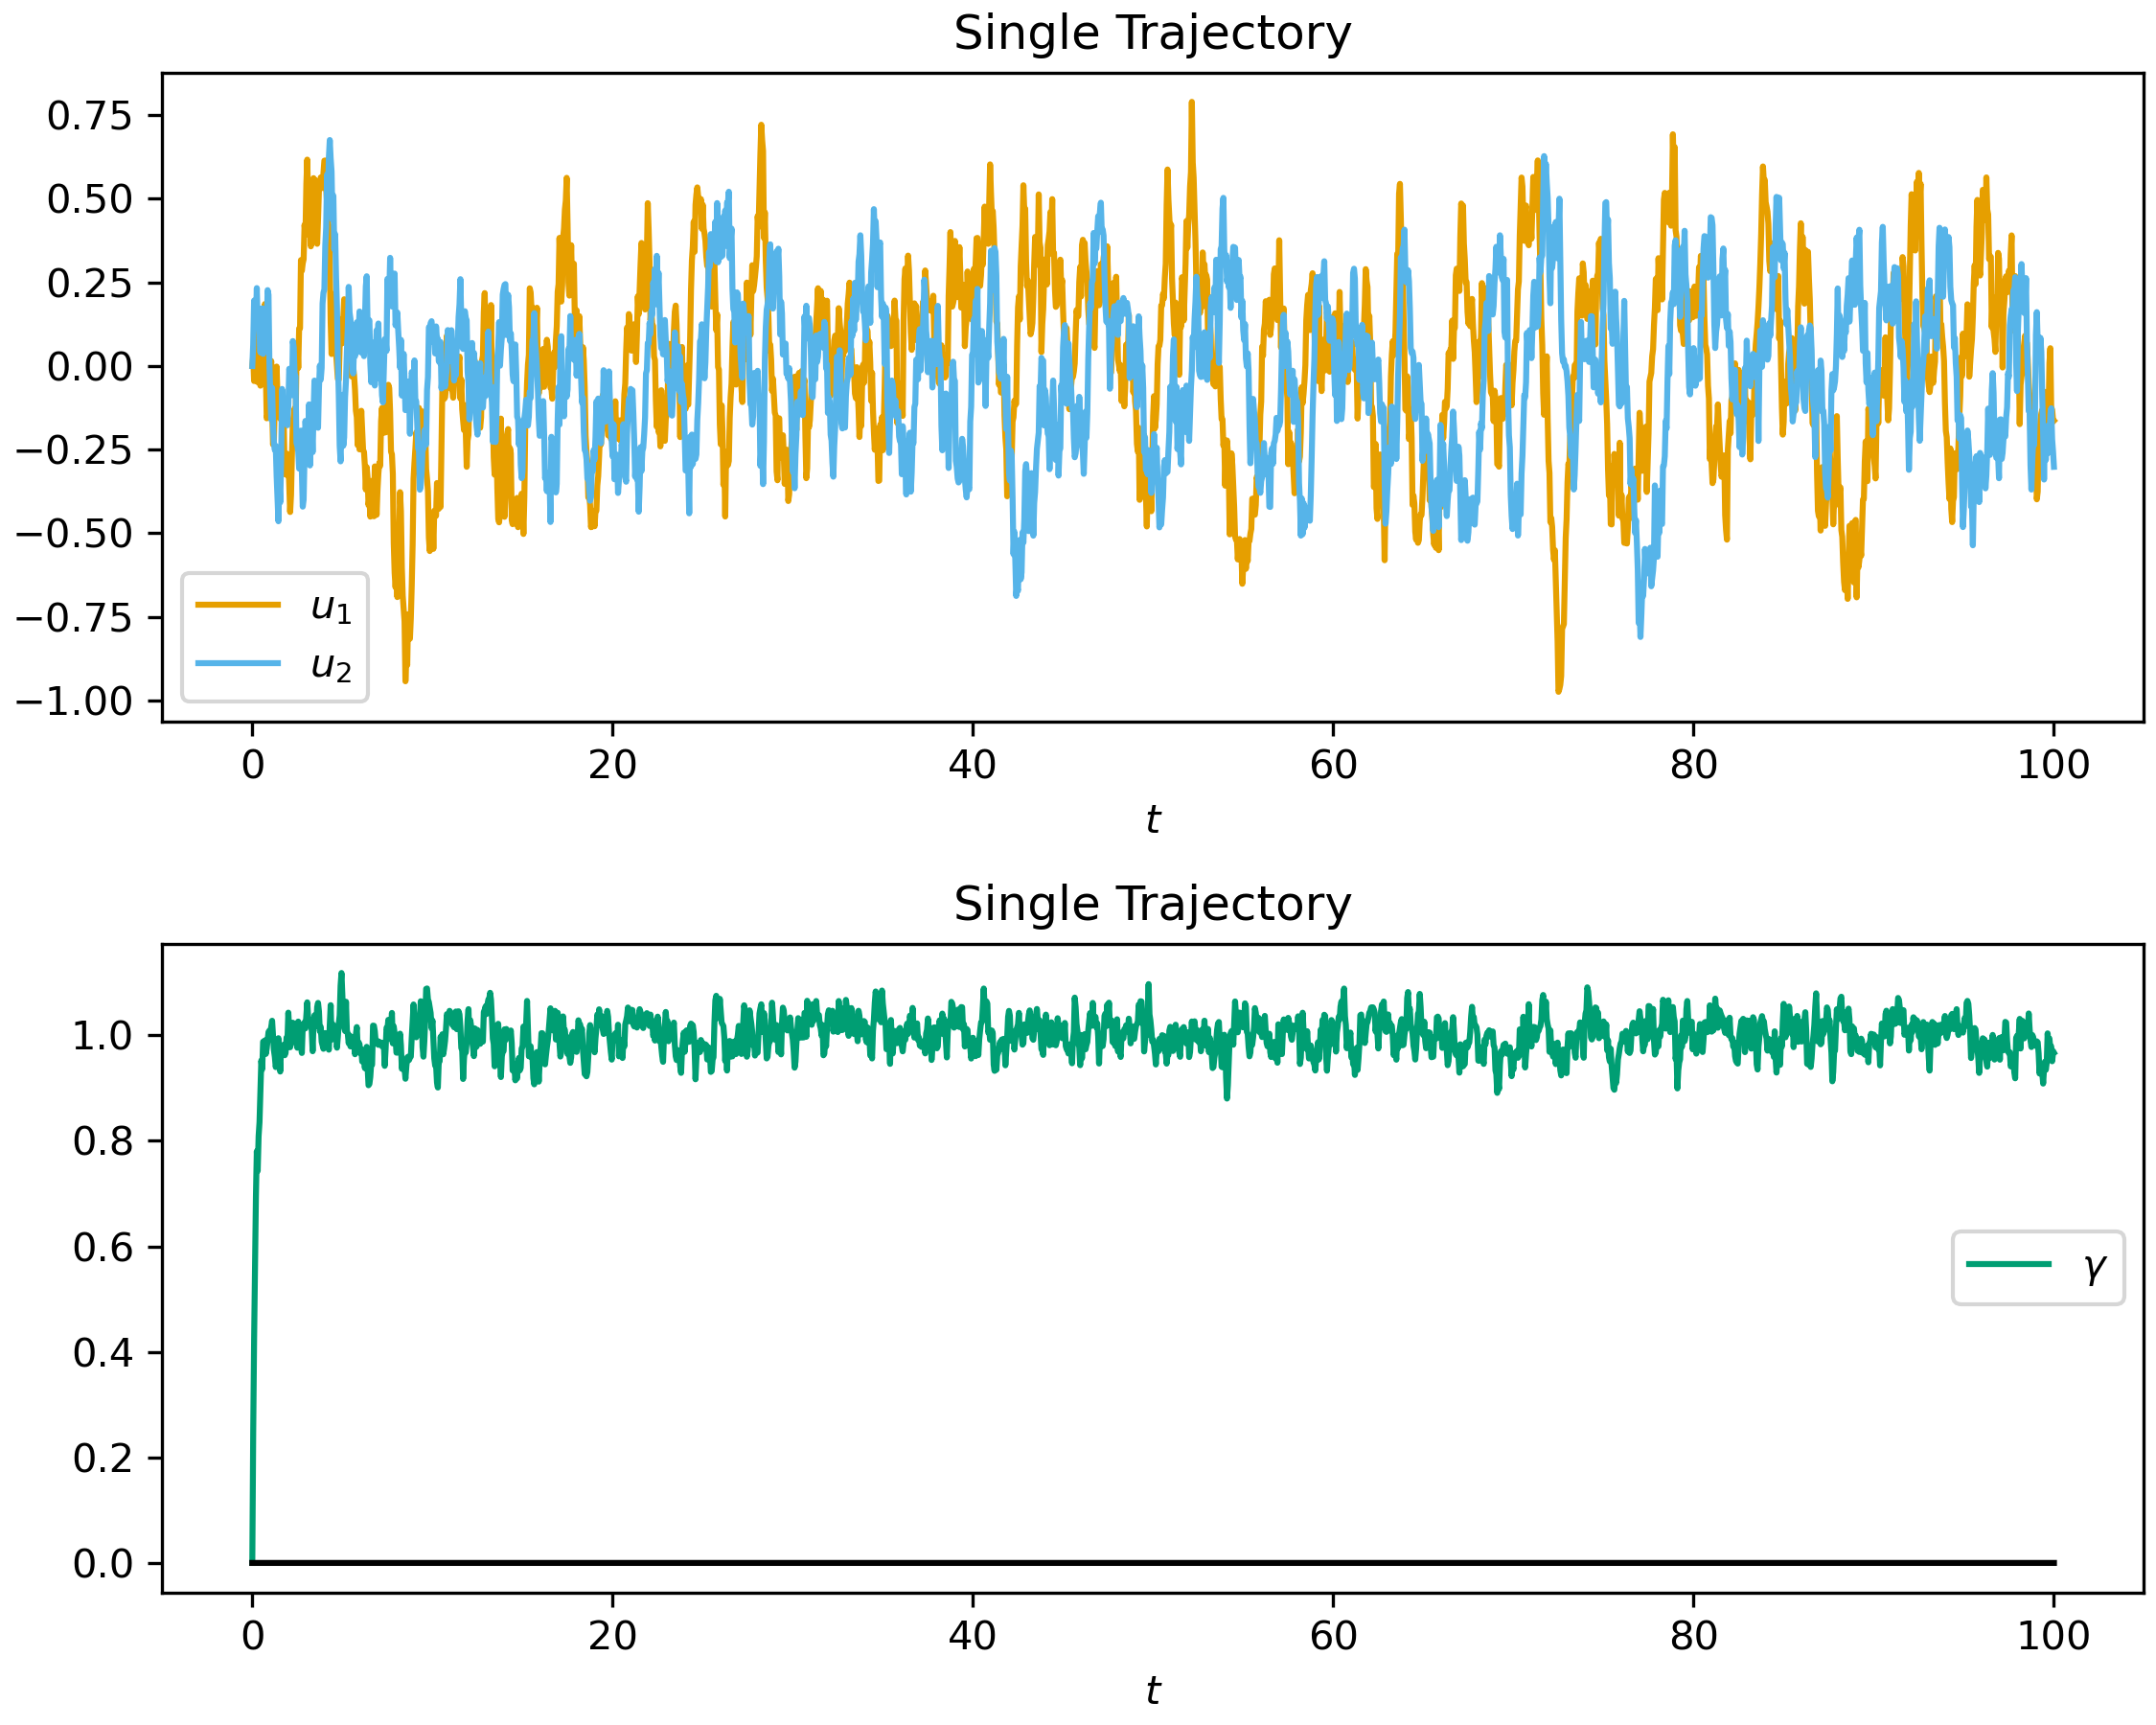
\includegraphics[width=0.75\textwidth]{../../src/2_traj_iii.png}
		\caption{A single realization of the linear SDE with multiplicative noise with the parameters $\omega = 1$, $\sigma_u = 0.5$, $d_{\gamma} = 4.8$, $\widehat{\gamma} = 1$, and $\sigma_{\gamma} = 0.1$ with initial condition $u = u_1 + i\,u_2 = v = 0$. For clarity of deciphering when $u_1$, $u_2$ are in a stable or unstable regime, we include a solid black line at $\gamma = 0$.}
		\label{fig:2_traj_iii}
	\end{figure}

	\begin{figure}[H]
		\centering
		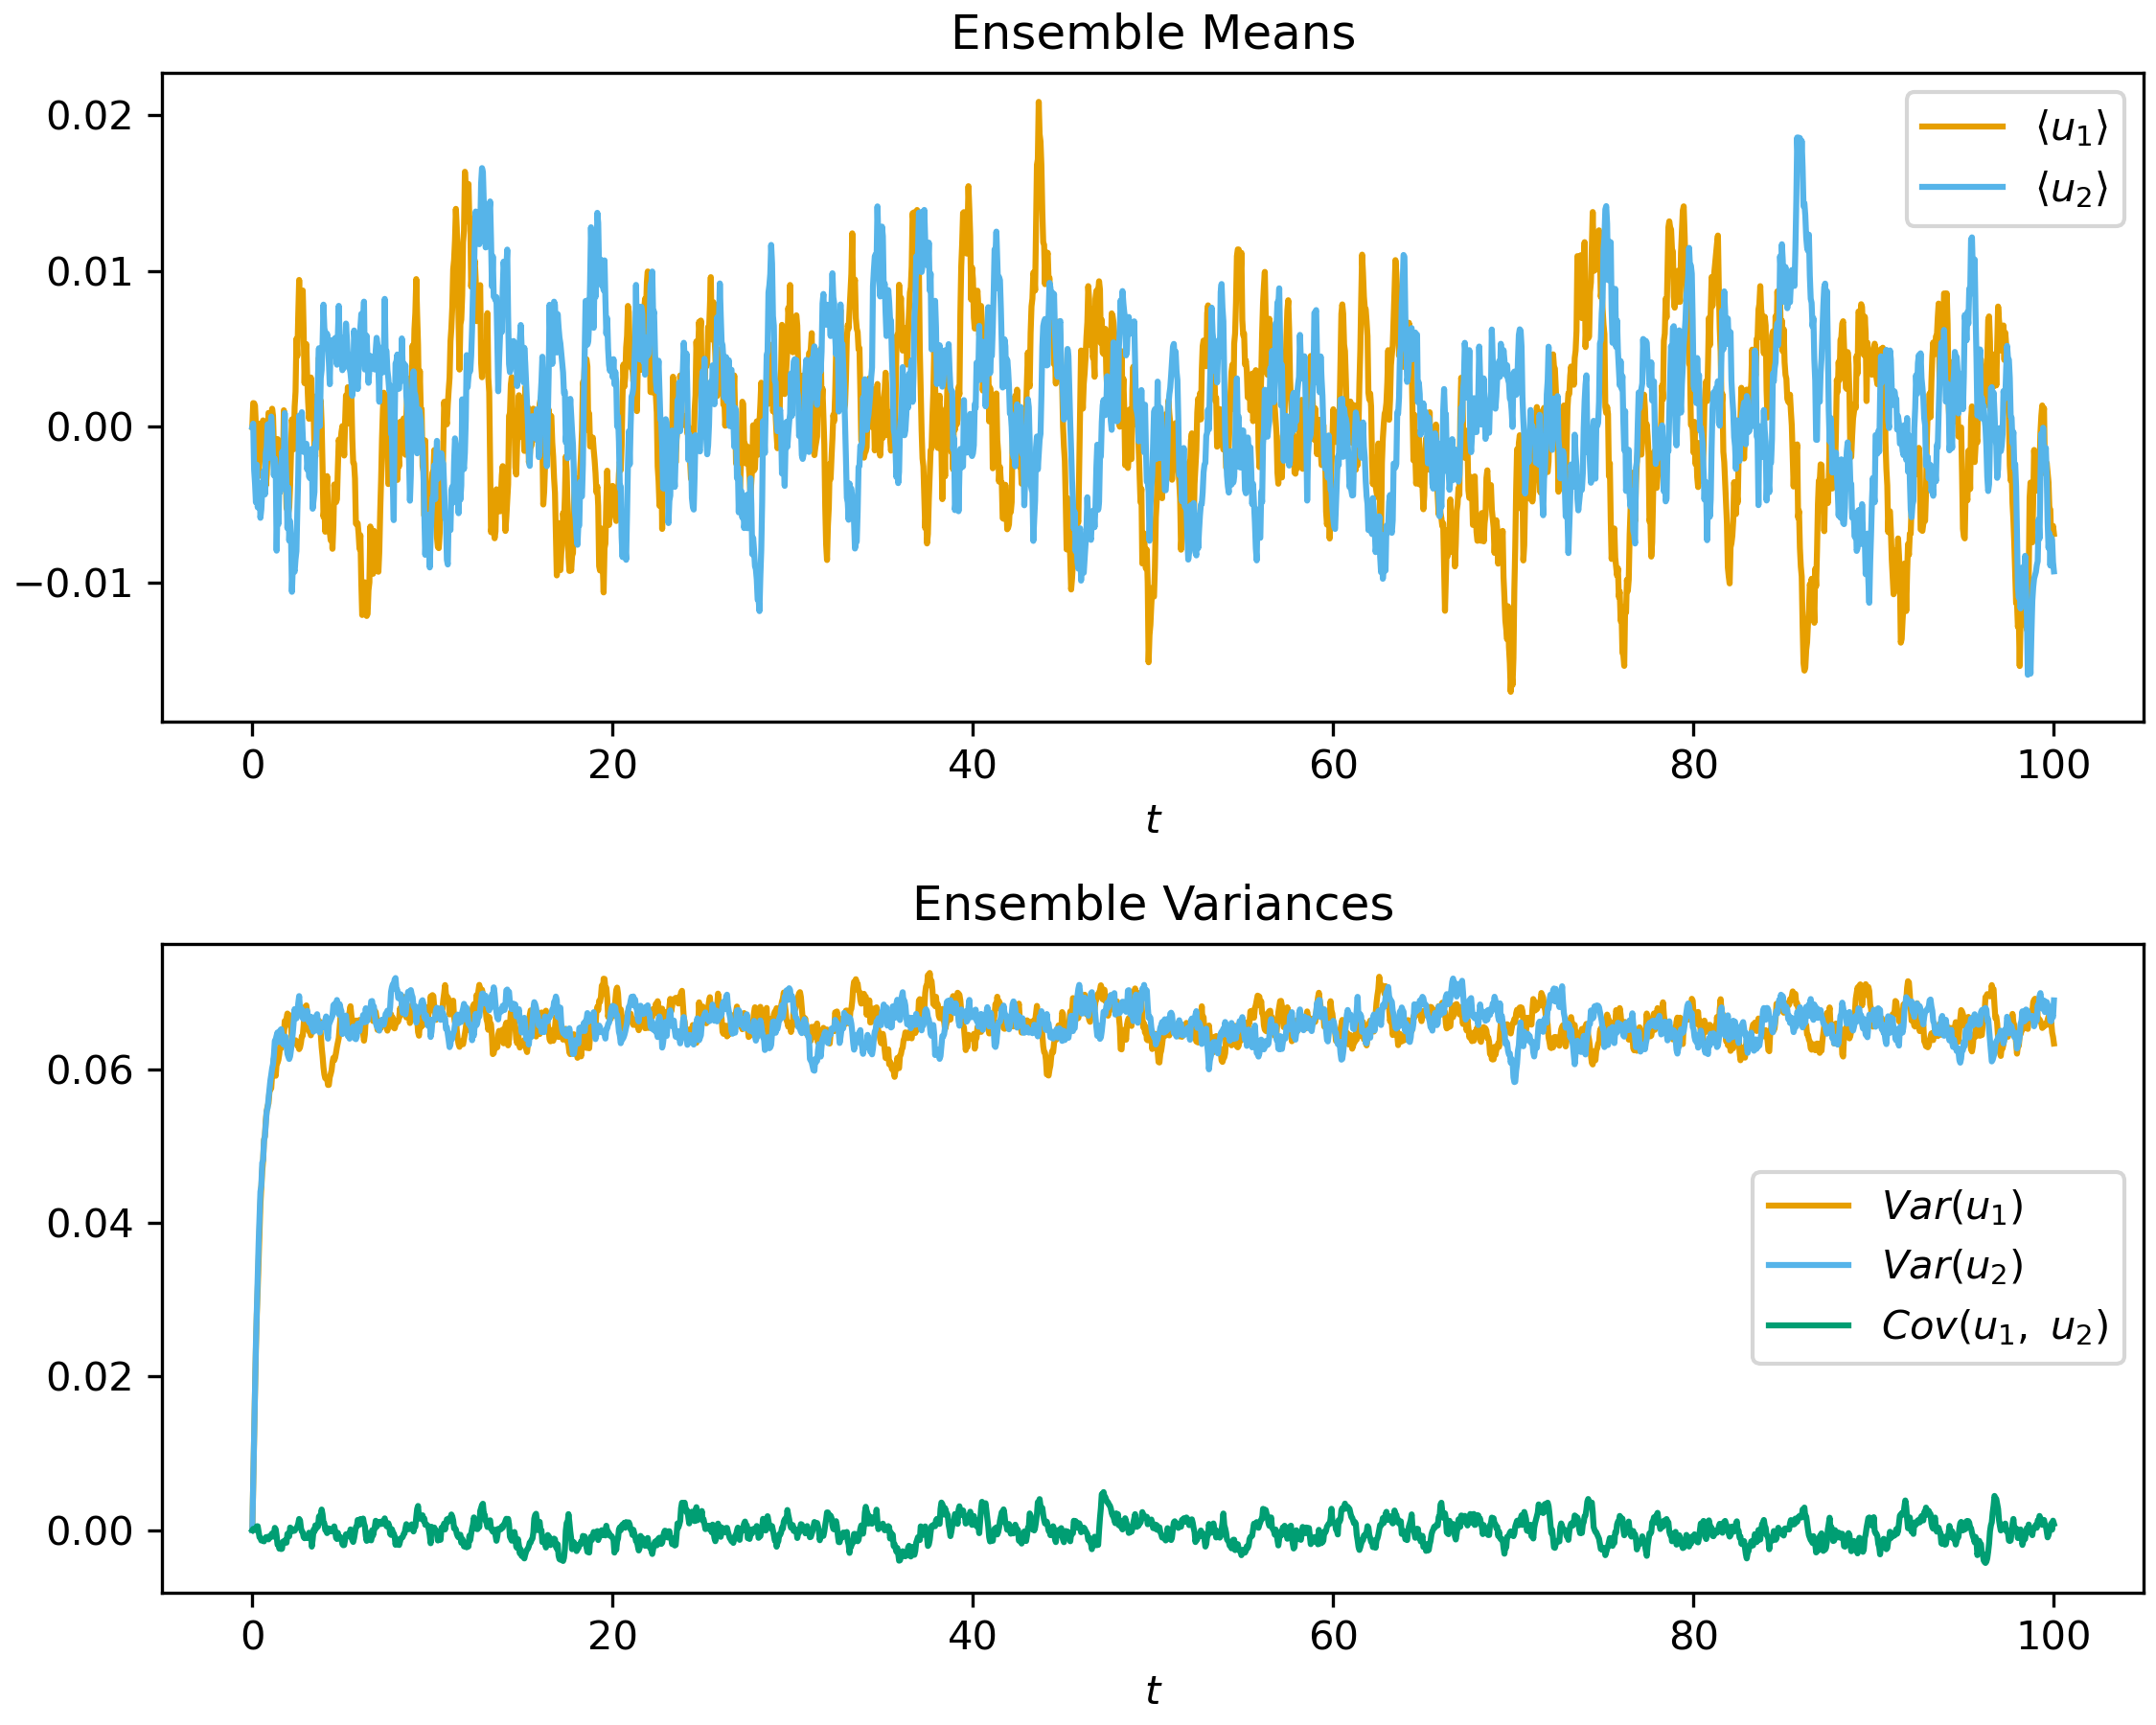
\includegraphics[width=0.75\textwidth]{../../src/2_ens_stats_iii.png}
		\caption{The ensemble statistics for 1000 realizations of the linear SDE with multiplicative noise with the parameters $\omega = 1$, $\sigma_u = 0.5$, $d_{\gamma} = 4.8$, $\widehat{\gamma} = 1$, and $\sigma_{\gamma} = 0.1$ with initial condition $u = u_1 + i\,u_2 = v = 0$ for each realization.}
		\label{fig:2_ens_stats_iii}
	\end{figure}
	
	\begin{figure}[H]
		\centering
		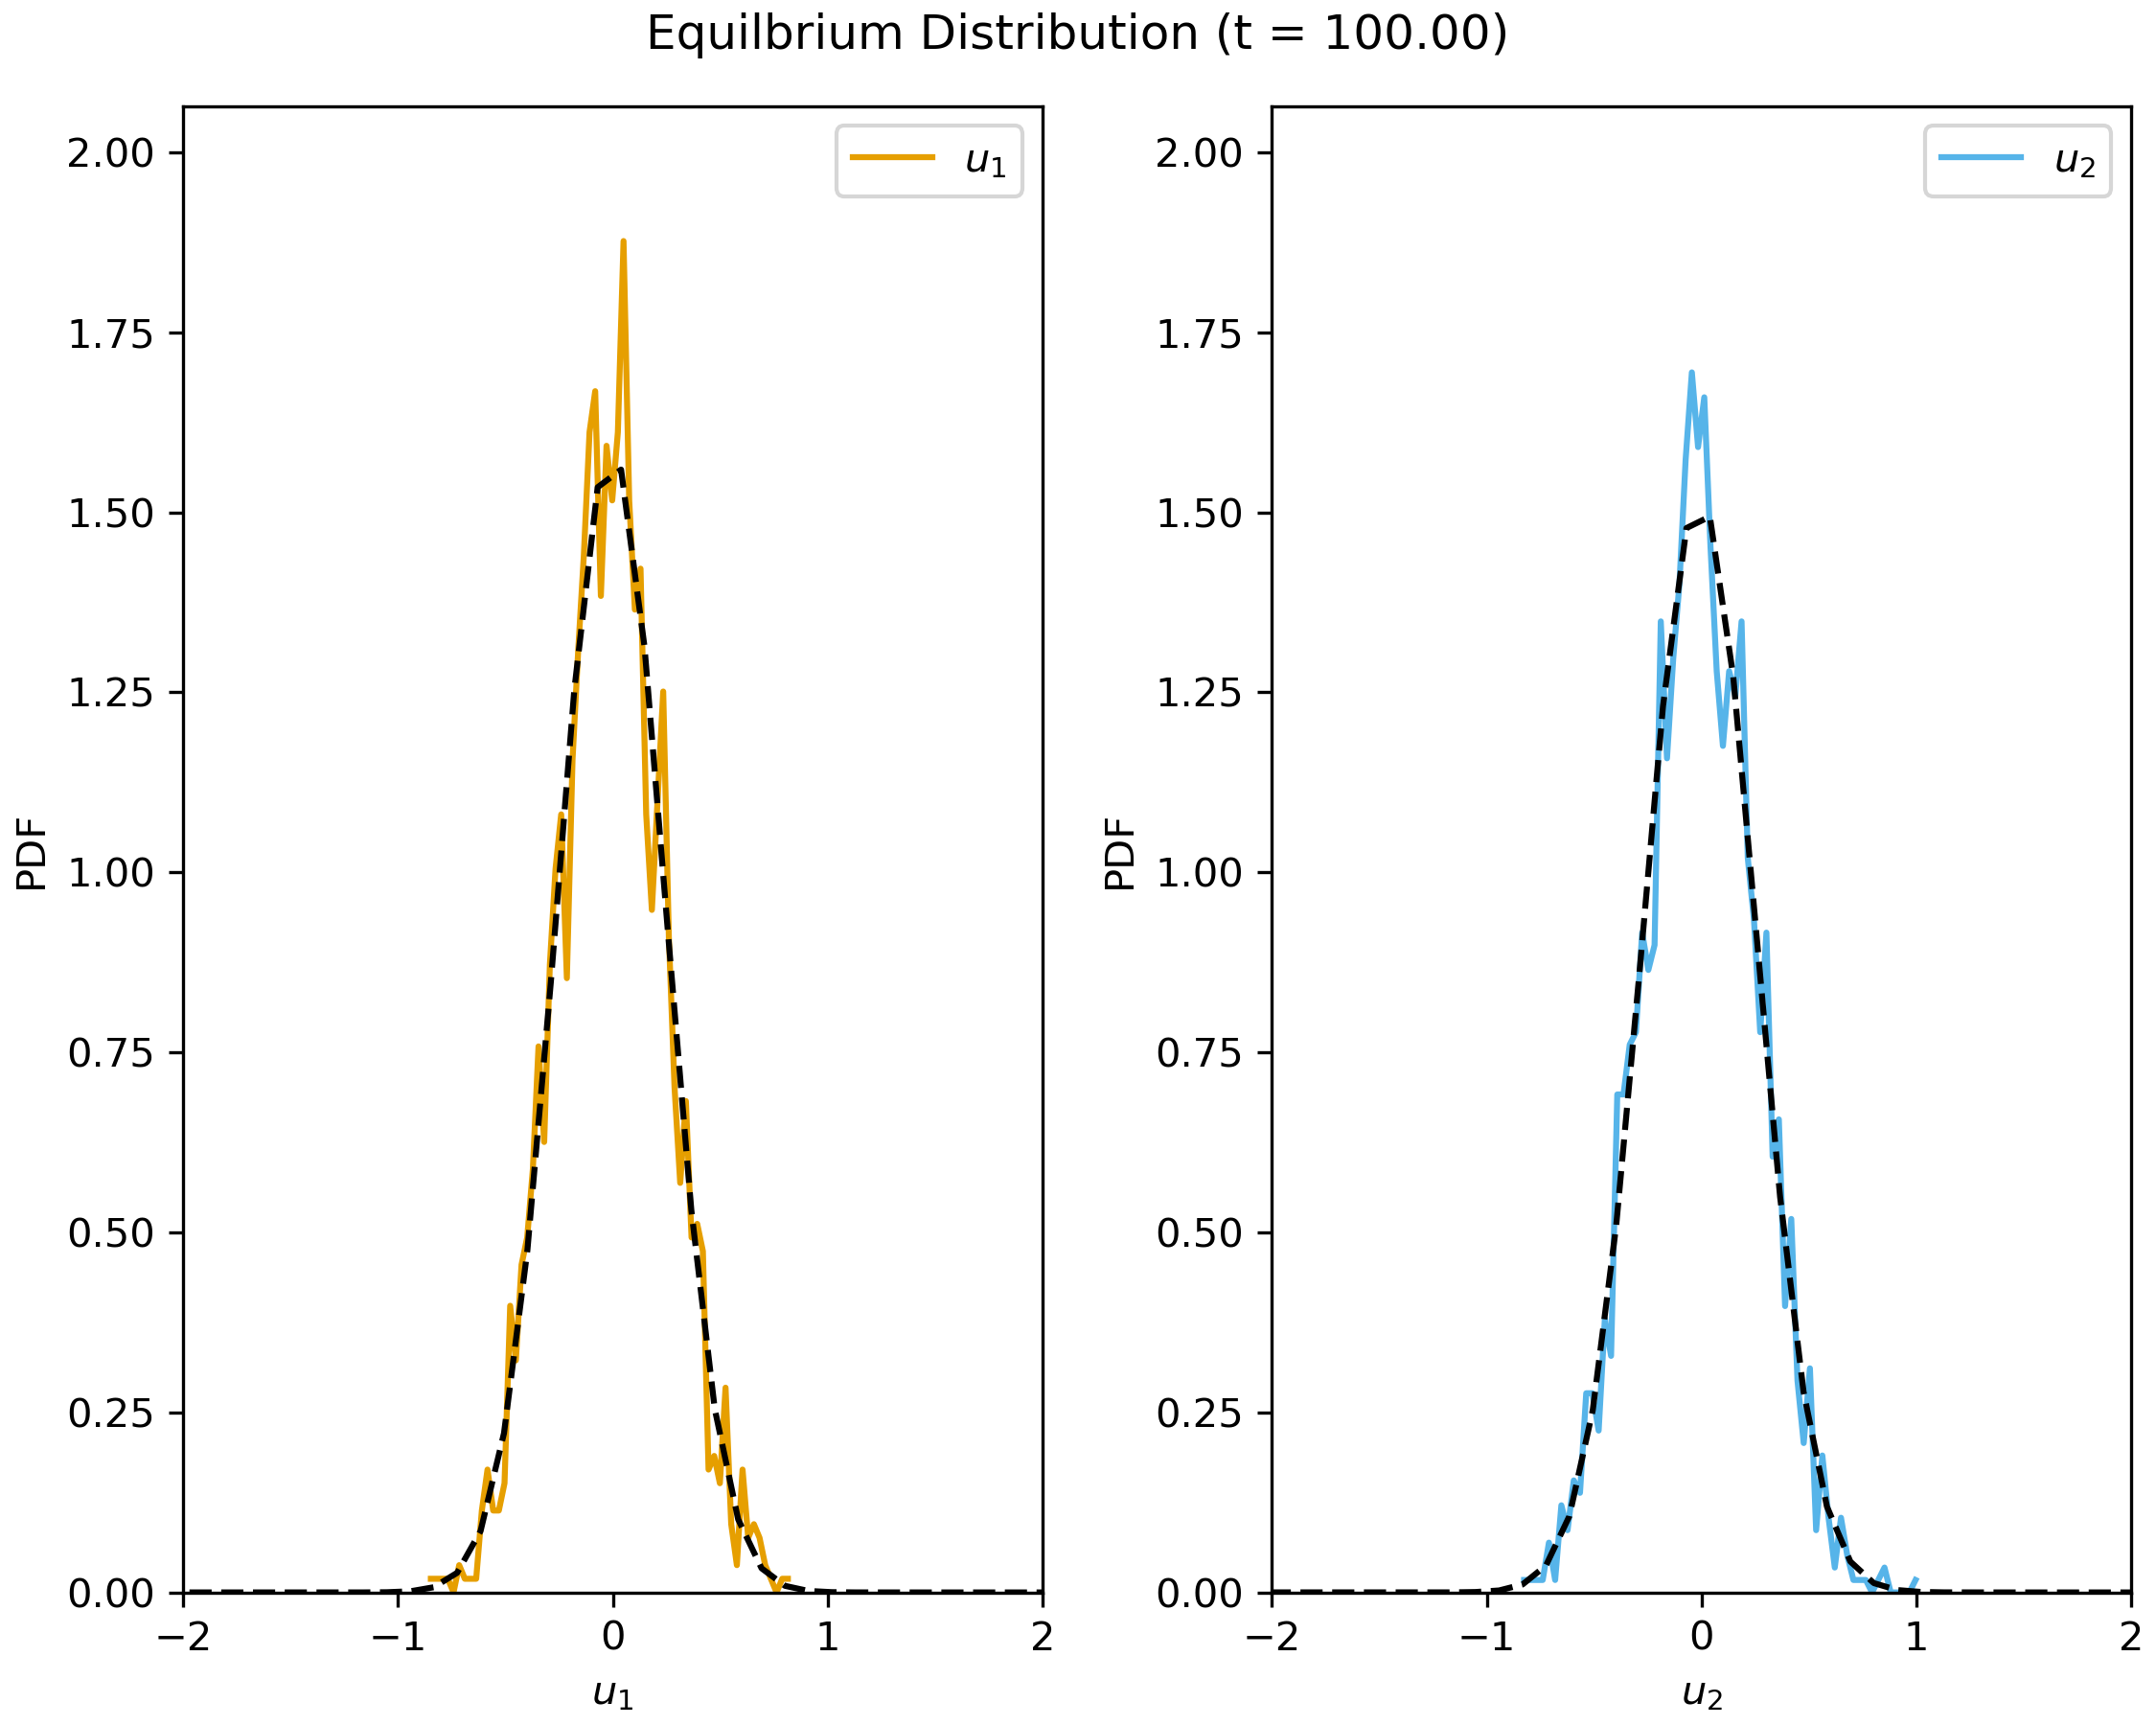
\includegraphics[width=0.75\textwidth]{../../src/2_equ_pdf_iii.png}
		\caption{The equilibrium distribution for 1000 realizations of the linear SDE with multiplicative noise with the parameters $\omega = 1$, $\sigma_u = 0.5$, $d_{\gamma} = 4.8$, $\widehat{\gamma} = 1$, and $\sigma_{\gamma} = 0.1$ with initial condition $u = u_1 + i\,u_2 = v = 0$ for each realization. The dashed black line corresponds to a Gaussian fit for the data.}
		\label{fig:2_equ_pdf_iii}
	\end{figure}
	
	\begin{figure}[H]
		\centering
		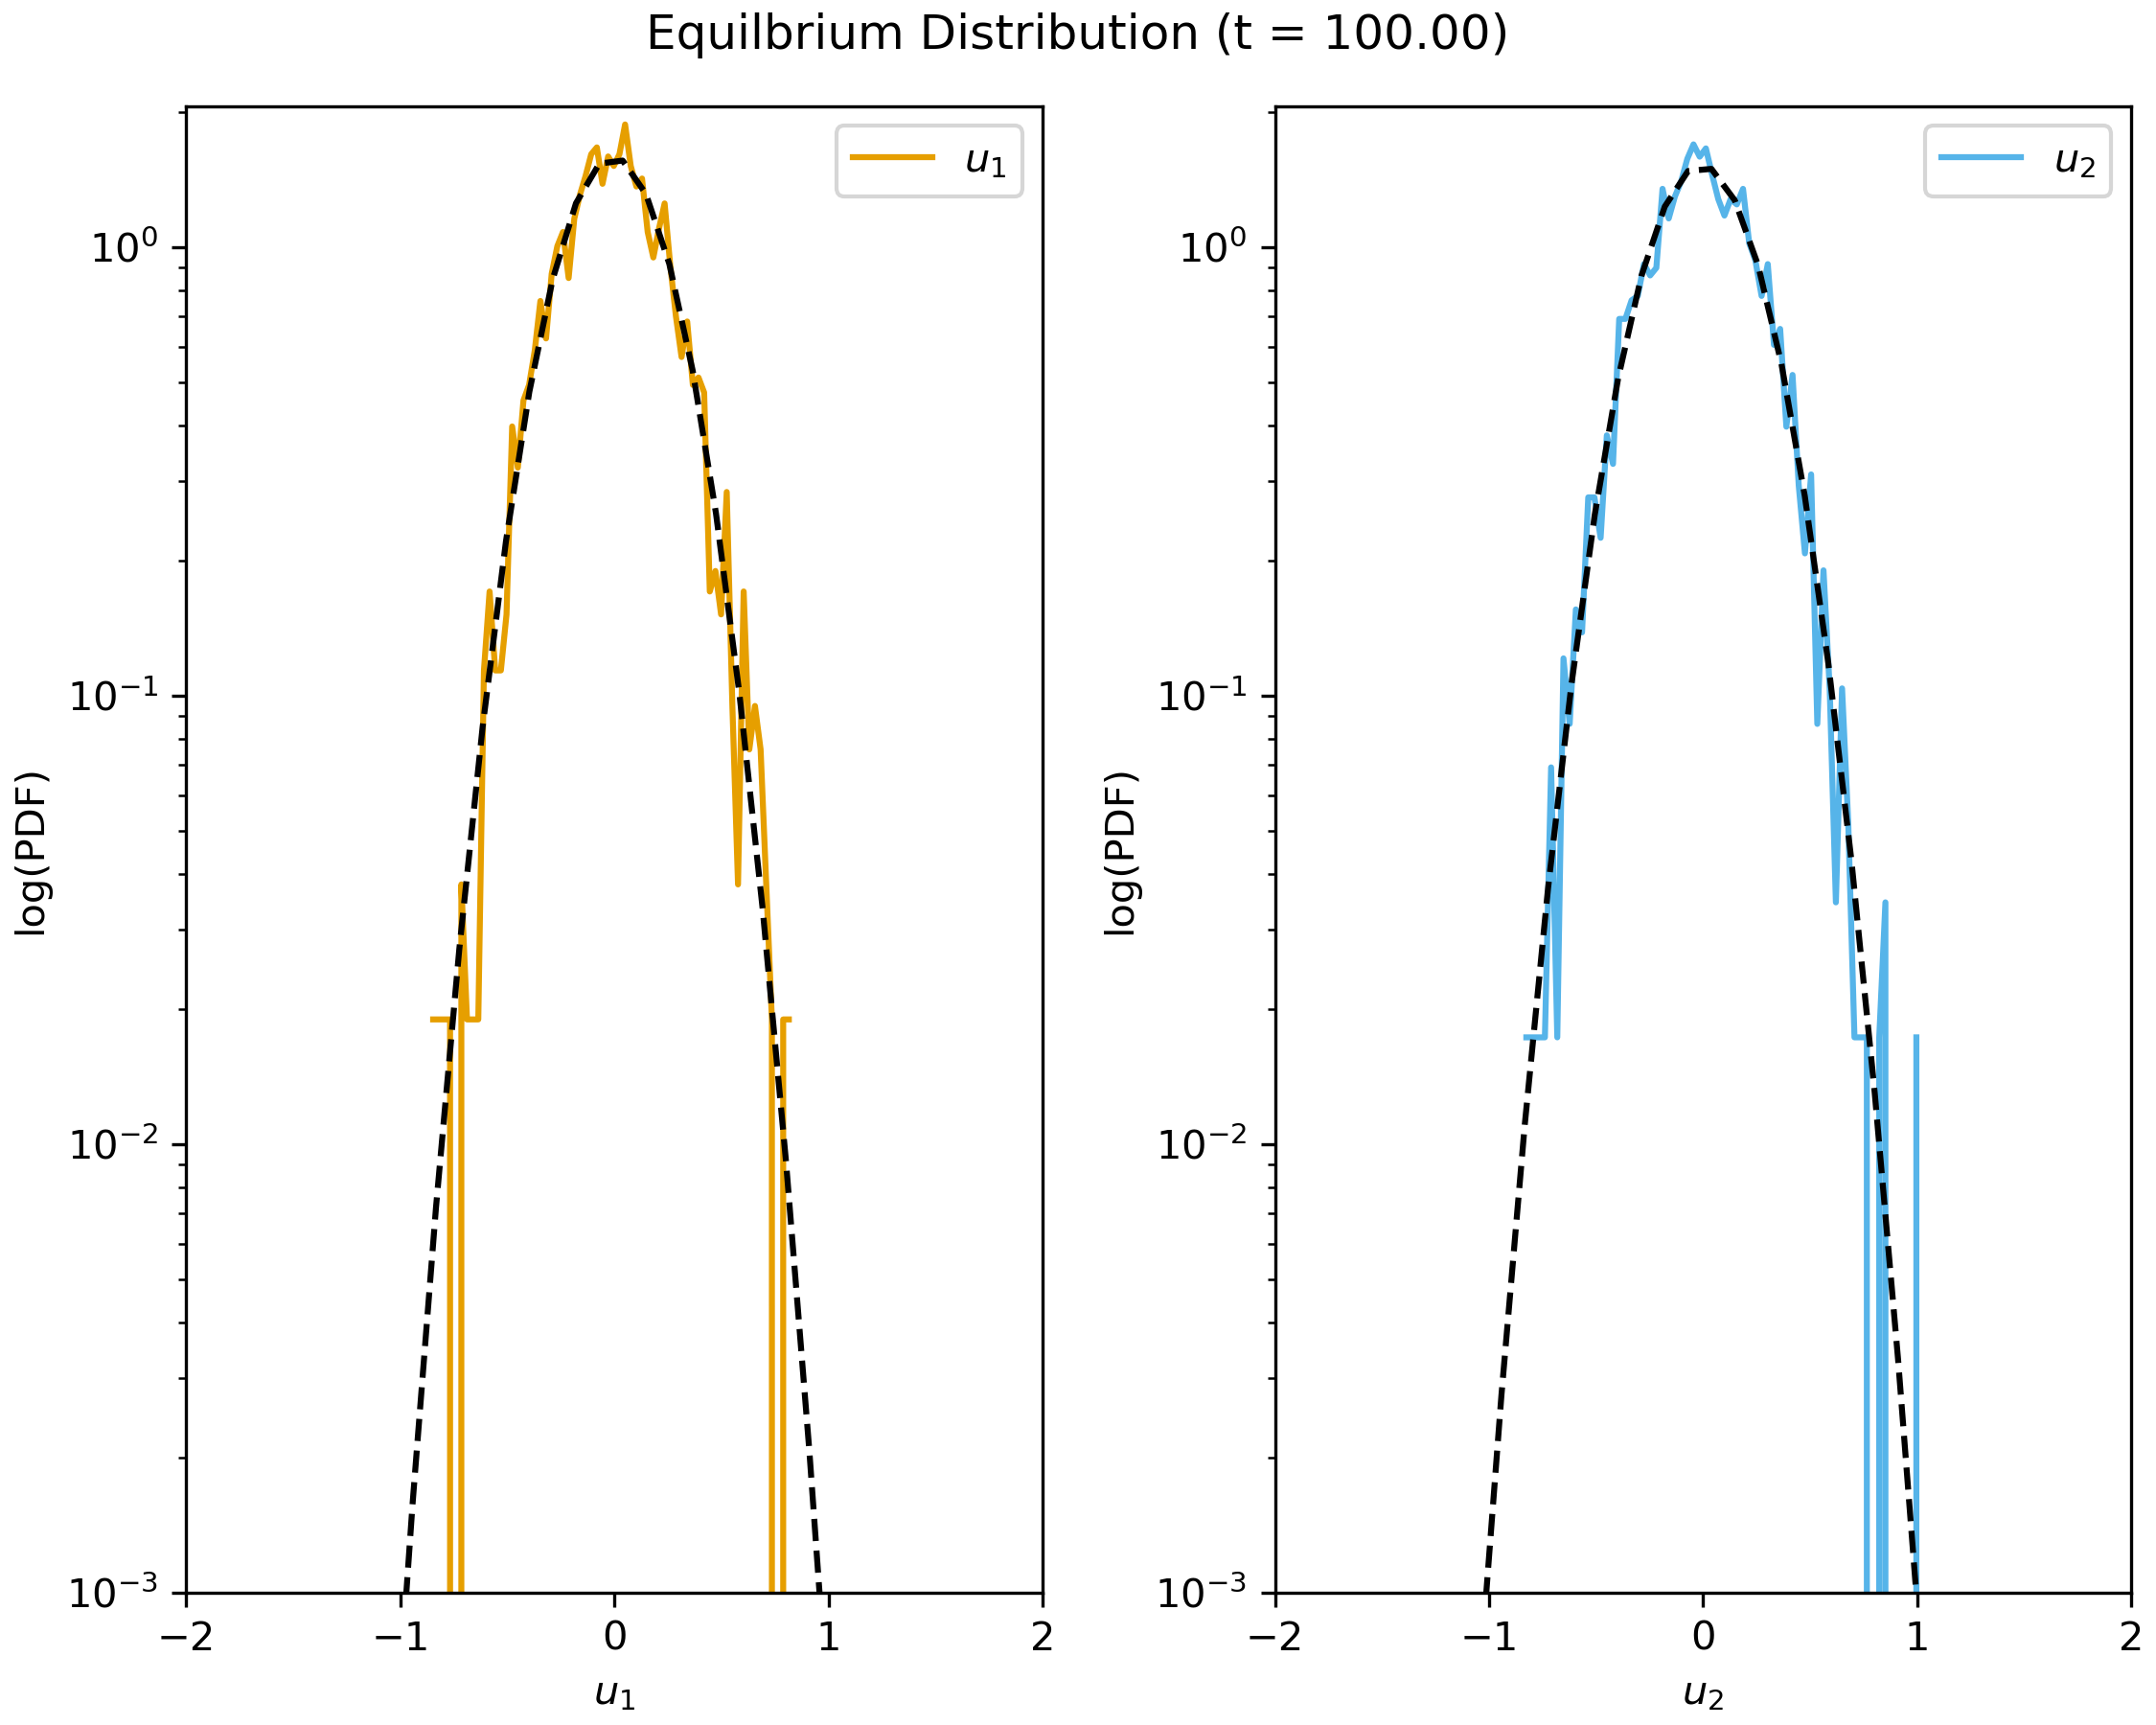
\includegraphics[width=0.75\textwidth]{../../src/2_log_equ_pdf_iii.png}
		\caption{The log of the equilibrium distribution for 1000 realizations of the linear SDE with multiplicative noise with the parameters $\omega = 1$, $\sigma_u = 0.5$, $d_{\gamma} = 4.8$, $\widehat{\gamma} = 1$, and $\sigma_{\gamma} = 0.1$ with initial condition $u = u_1 + i\,u_2 = v = 0$ for each realization. The dashed black line corresponds to a Gaussian fit for the data.}
		\label{fig:2_log_equ_pdf_iii}
	\end{figure}

\end{enumerate}

Source code is available from the GitHub repository
	
	\begin{center}
		\url{https://github.com/jasonltorchinsky/MATH833_HW/releases/tag/hw4}
	\end{center}

	and is given in Appendix~\ref{app:code_2}. In short, the code takes a input parameters \texttt{-{-}omega}, \texttt{-{-}sigma\_u}, \texttt{-{-}d\_gamma}, \texttt{-{-}gamma\_hat}, \texttt{-{-}sigma\_gamma}, and \texttt{-{-}regime} which correspond to $\omega$, $\sigma_{u}$, $d_{\gamma}$, $\widehat{\gamma}$, $\sigma_{\gamma}$, and a name for the regime $u$ is in given those parameters, respectively. The code then simulates 2000 individual realizations of the linear SDE with multiplicative noise using the Euler--Maruyama method, and generates the included plots.
